\chapter{Physically-Informed Operational Robotic Trajectories for Scientific Expeditions}

\td{short premise here that also highlights publications}

\section{Introduction}
Transient, dynamic phenomena---deep-sea hydrothermal plumes, algal blooms, warm core eddies, lava flows---are of interest in many disciplines of observational science. \emph{Expeditionary science} encapsulates the observational sciences that require \emph{in situ} sample collection of environmental phenomena for scientific discovery and model development. In such cases, the environmental targets are typically impossible to observe using remote sensing (e.g., satellites) either due to desired spatial and temporal resolution, environment adversity (e.g., the deep sea, within closed structures), or the nature of the scientific target of interest and corresponding sensing equipment (e.g., building a taxonomy of algae requires physically processing water samples). Expeditionary science is, by definition, conducted in a partially-observable environment, and creating comprehensive pictures of these environments is further complicated by spatiotemporal distributions of dynamic phenomena. 

In this article, we study robot autonomy for charting deep-sea hydrothermal plumes, a particular class of scientific spatiotemporal phenomena. Understanding the fate of chemicals and particulates in hydrothermal plumes is of significant interest to biogeochemists and physical oceanographers; however, directly studying plumes in the water column is a substantial challenge. Hydrothermal plumes are driven by density differences between super-heated fluid at seafloor geothermal vents and the cold background seawater, creating a buoyancy force that causes the vent fluids to rise. The plume is typically chemical and particulate rich, and while rising through the water column, mixes (entrains) with the background seawater until it reaches a point of neutral buoyancy with the ambient seawater. At the neutrally-buoyant layer, fluid from the plume spreads out in a large plane (following an isopycnal of constant density). From this layer, metals, sediment, and other suspended particulates carried by the plume may drop out and be redeposited onto the seafloor, and any persisting chemicals diffused or digested by microbes. A robot tasked with charting a plume must be able to forecast where and when it will intersect with different parts of the plume in order to collect useful observations of its spatiotemporal structure, but the state is uncertain as a result of unseen advective forces (e.g., deep currents, topographic updrafts), diffusive mixing, and unknown venting characteristics that dictate plume formation. Point \emph{in situ} measurements in a continuous three-dimensional volume over time make the problem worse, as no single measurement is sufficient to locate the plume. 

In addition to the technical challenges of determining a sensing strategy in the face of highly uncertain and dynamic phenomena, robot operational constraints also create planning challenges. In the expeditionary sciences, and particularly within deep-sea research, mobile robots equipped with multi-sensor payloads are increasingly used to perform surveys in these dynamic environments, typically executing preset trajectories hand-designed by human scientists (e.g., \cite{camilli2010tracking}). In this mode, the robot cannot react to measurements while executing the set trajectory. Although in dynamic environments such open-loop trajectories can result in sparse measurements of the target phenomenon (plume) or can miss short-lived events entirely \cite{flaspohler2019information}, this concept of operations remains the state-of-the-art in practical deployments due to their relative ease to encode, limited computational capacity of the platforms, and predictability of robot actions to outside supervisors. In this article, we consider constraints introduced by a specific robot, autonomous underwater vehicle (AUV) \emph{Sentry}. This AUV, operated by the National Deep Submergence Facility (NDSF) at the Woods Hole Oceanographic Institution (WHOI) \cite{kaiser2016design}, by operational policy is only permitted to execute pre-determined regular trajectories like ``lawnmower'' patterns or spirals, making online adaptation impossible.

Enabling robots like \Sentry to collect scientific observations of spatiotemporal phenomena while operating without access to adaptive behaviors requires an autonomy system that can place operationally-approved fixed trajectory patterns strategically to maximize desirable intersections with the phenomena. To be able to strategize effectively, a means of learning to forward simulate the dynamics of the target environment over a long-horizon from a small history of robot deployments is required. This is fundamentally a \emph{sequential decision-making problem}, and is closely related to informative path planning (IPP), in which a robot selects behaviors according to an information-theoretic reward function computed over a probabilistic belief of the environment state. Existing methods in IPP (e.g., \cite{Hitz2017,hollinger2013sampling,flaspohler2019information,levine2010information,binney2012branch}), the related field of experimental design and optimal sensor placement (e.g., \cite{krause2008near,wang2019reinforcement}), and general decision-making under uncertainty (e.g., \cite{sunberg2018online, somani2013despot,kocsis2006bandit,Silver2010}) have demonstrated how sequential decision making can be applied to sampling scenarios in which online, adaptive behaviors are possible, the phenomenon of interest is static, and/or there is an opportunity to train the belief model from many trials, multiple sensors, or highly adaptive trajectories. Each of these typical scenarios is violated for the expeditionary science sampling problem---online adaptation is not possible, the phenomenon is dynamic, and there are very few total number of deployments for model training. 

We directly address the open challenges of sample-efficient dynamics learning and few-step planning sequences under operational constraints unaddressed by the classical informative path planning frameworks with our novel \emph{deployment-by-deployment} sequential decision-making formulation for expeditionary missions, \PHORTEX: \phortex (Fig.~\ref{fig:intro_summary}). In \PHORTEX, each deployment of the AUV is considered a single action, and each action is composed of a chain of operationally-approved trajectory patterns (e.g., lawnmowers) parameterized by a small set of characteristics (e.g., orientation, origin, resolution). The chain parameters are jointly optimized over a long-range forecast of the spatiotemporal distribution of interest (e.g., plumes) to maximize expected intersections with a moving plume. These forecasts are provided by our probabilistic model \PHUMES: \phumes, which uses an embedded analytical simulator (e.g., numerical model of buoyancy-driven plumes) as an inductive bias for tractable dynamics learning, and can be incrementally trained from any data available from prior deployments or from opportunistic use of sensors deployed as part of normal expedition operations. The rest of this introduction provides further detail on the challenge of charting hydrothermal plumes and deploying robots at sea, and concludes with a statement of contributions related to our formulations of \PHORTEX and \PHUMES. 

\begin{figure}[h!]
    \centering
    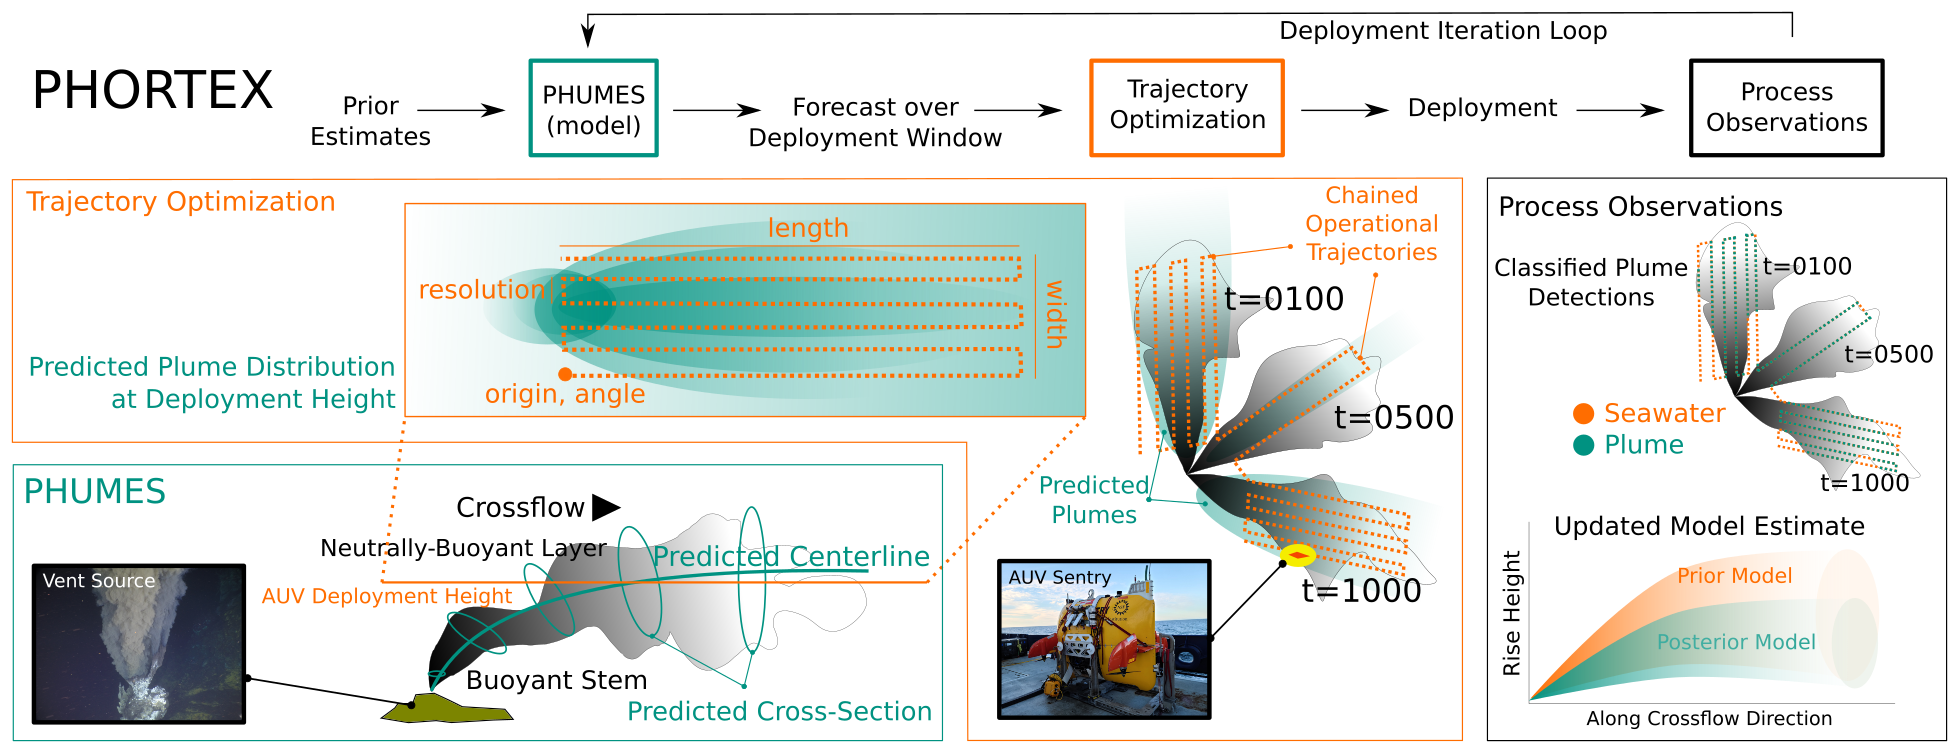
\includegraphics[width=\columnwidth]{figures/summary_intro_figure_v2.png}
    \caption{An overview of \PHORTEX: \phortex. Over the course of an expedition, an autonomous vehicle is deployed several times. In preparation for a deployment, \PHUMES is used to generate a probabilistic forecast of the target spatiotemporal distribution. \PHUMES can be seeded with prior information from scientific knowledge, data of opportunity from other deployed sensing equipment, or previous robot deployments. A trajectory optimizer is given the forecasts and modifies the parameters of a trajectory primitive. Several primitives are chained together to form a complete deployment trajectory. The robot is then deployed and executes the trajectory. Following a deployment, \emph{in situ} observations from multiple heterogeneous science sensors are collected from the robot and fused into a data product that can be used to train \PHUMES, and the deployment planning process iterates. Here, the task of hydrothermal plume charting with AUV \emph{Sentry} is illustrated. \PHUMES generates an forecast of temporally-evolving plume centerlines and cross-sections from estimates of vent characteristics and fluid crossflow (e.g., current) informed by measurements or prior distributions over these variables. For a given height that \emph{Sentry} can operate (and is constrained to operate for any given primitive), chains of uniform coverage lawnmowers are optimized (over parameters such as length, width, resolution, origin, and global angle) with respect to the plume forecast to intersect and track the plume over the course of a deployment window. Following a \emph{Sentry} deployment, observation locations are classified as binary plume detections from analysis of several science sensors. This product is then used to update the \PHUMES model of plume centerline and cross-section over time. The new \PHUMES model is then used to plan the next deployment of \Sentry.}
    \label{fig:intro_summary}
\end{figure}


%%%%%%%%%%%% Hydrothermalism
\subsection{Charting Deep-Sea Hydrothermalism}
\label{sec:charting-plumes}
Hydrothermal vents in the ocean were first observed in 1977 at the Galapagos Rift \cite{corliss1979submarine}, and since have been a concerted focus of geodynamical and biogeochemical studies. Venting sites, energized by magmatic sources, release fluids between 20-\SI{400}{\celsius} (background deep ocean temperatures are approximately \SI{2}{\celsius}) and imbued with minerals, metals, dissolved gases, and other compounds \cite{jannasch1985geomicrobiology, martin2008hydrothermal}. These warm, nutrient-pumping sites in the deep ocean have created oases of unique micro- and macro-fauna \cite{corliss1979submarine}. Detection and characterization of seafloor hydrothermal venting are critical for understanding fundamental interactions between the deep ocean, its underlying basaltic crust, the deep biosphere, and (bio)geochemical fluxes.

We build on a wealth of work that has primarily focused on localizing hydrothermal venting plume sources (e.g., \cite{jakuba2007stochastic, mcgill2011robot, nakamura2013discovery, paduan2018discovery, mason2020evaluation, wang20203, kim2020discovery,ferri2010novel}) using a variety of equipment such as ship-based acoustics, towed instrument rosettes, remotely-operated vehicles (ROVs), submersibles, and autonomous underwater vehicles (AUVs). Generally, these methods use detections of anomalous water masses (as determined from \emph{in situ} sensors) to constrain the location of a seafloor vent for specialized seafloor equipment to be subsequently deployed to e.g., estimate bulk chemical or nutrient flux from the vent or characterize the driving magmatic system underneath the crust. The localization methods can be fully offline, in which surveys by vehicles like \Sentry with no adaptive capacity are post-processed and estimates of vent locations are inferred from a single survey \cite{jakuba2007stochastic,nakamura2013discovery}, or fully online, in which autonomous gliders with adaptive capabilities utilize gradient descent of similarly myopic adaptive sampling strategies to seek a plume source are used \cite{wang20203}. In \cite{branch2020demonstration}, an autonomous glider tasked with localizing a vent source could adaptively chain uniform coverage trajectories together with increasingly fine resolution as the robot position converged on an estimate of a plume source location while underway. We emulate this chaining methodology in our trajectory chaining scheme, however the selection of trajectories by \PHORTEX is done completely offline before AUV \Sentry is deployed. Indeed, it is notable that online strategies for hydrothermal plume hunting almost universally employ glider-type robot platforms, which are typically smaller, payload-limited, and less depth-capable than vehicles like \Sentry. 90\% of known vent fields are deeper than \SI{200}{\meter} in the ocean, and over 75\% are deeper than \SI{1000}{\meter} \cite{beaulieu2013authoritative}. State-of-the-art gliders are typically not rated deeper than \SI{1000}{\meter}, which means that deep-sea research of the majority of vent sites are reliant on vehicles like \Sentry and demand advances in offline-suited planning techniques.

We also draw on ``plume hunting'' research in robotics, which has been equivalently styled as odor mapping, odor localization, source localization, and source seeking. In these works, the ``source'' could be any type of emitting site (e.g., gas, radio, acoustic, odor) and through partial observations of the emitted substance, the source is discovered using techniques that can be divided broadly into biologically-inspired heuristic search (e.g., \cite{reddy2022olfactory,chen2019odor}) or adaptive informative path planning (e.g., \cite{salam2019adaptive}). Biological or heuristic techniques draw (varying-levels of) inspiration from animal or insect behavior in olfactory settings. Such techniques typically include gradient-based algorithms like chemotaxis \cite{morse1998robust}, or algorithms that directly mimic a particular animal \cite{edwards2001representing}. These techniques are typically reactive and myopic, although they have been demonstrated to be relatively robust in open-world settings. In contrast, adaptive informative path planning can be nonmyopic, and typically attempts to embed knowledge (either heuristically or rigorously) about flow-fields (i.e., advection and diffusion) to assist in plume localization. Such techniques also live on a spectrum, from algorithms that resemble biologically-inspired techniques like infotaxis \cite{vergassola2007infotaxis} to methods that use model order reduction techniques (like proper orthogonal decomposition) to encode complex numerical models (like the Navier-Stokes equations) into a belief model to better treat complex data \cite{peng2014dynamic}.

While source discovery remains an important area of research, in this article we focus on how science can be advanced at the hundreds of vents that have been successfully identified. Thus, we pose a complementary problem to source discovery: \emph{given a venting source, what impact do the venting fluids have on the local environment?} In this framing, rather than using detections of a plume as a means of source localization, the detections themselves are the valuable data product for scientific inquiry. By placing instruments throughout an evolving plume structure over multiple length- (meter to kilometer) and time- (hours to days) scales to collect dense in-plume measurements, previously intractable questions with respect to microbial lifecycle and transport, carbon cycling, and anomalous water mass formation, can be approached. Work that has used robots to map or chart plume-like structures has been presented as the ``front-tracking'' problem \cite{li2014multi,chen2019odor}. In this problem, two water masses converge (such as the warm hydrothermal fluid and the cold background seawater), and the goal is to use a robotic vehicle to track the edge of these water masses or stay within a single type of water mass. The importance of both multirobot collaboration and online decision-making in these schemes is essential to their efficacy; as far as we are aware, this article is the first to present a water mass tracking solution within an offline optimization strategy with a single agent, and the first to attempt this for the hydrothermal charting problem.

%%%%%%%%%%55 Logistics
\subsection{Closing the Loop: Expedition Logistics for Deep-Sea Robotics}
Oceanographic research expeditions are an undertaking that requires the coordination and collaboration of a science party, external engineering teams that maintain and operate the scientific equipment used during studies, and the captain and crew aboard a research vessel (on which everyone lives and works during operations). Deep-sea (depths below the mesopelagic zone starting at \SI{1000}{\meter}) capable robotic platforms used in oceanic research are assets independently maintained from a ship, and typically requested on a per-expedition basis. AUV \Sentry may be deployed on tens of expeditions in a given year, with up to 250 days at sea. Safety of both people and equipment are held to the highest importance. Further, the critical role of \Sentry in oceanographic research drives the strict operational policies that dictate \Sentry deployments to prevent vehicle loss or damage.

It is with this context that \Sentry deployments are designed by the science party and ultimately approved by the \Sentry engineering team. In a typical workflow, the science party may provide a set of coordinates or waypoints they generate based on bathymetric maps, prior knowledge, or previous data (when available). The \Sentry team design survey trajectories based on these coordinates and respecting basic operational constraints of the vehicle (e.g., speed, minimum/maximum altitude from the seafloor). With approval of the \Sentry team, science party, and captain, the survey is then executed. A single ``dive'' of \Sentry is multiple hours (typically not less than 5 hours, and under 24 hours). At the conclusion of a dive, \Sentry is recovered from the ocean and data products containing hundreds of thousands of point measurements from multiple heterogeneous sensors are made available to the science team within a few hours after \Sentry returns to the deck. Depending on the length of the dive, 12-18 hours of vehicle cycling time (e.g., recharging, instrument maintenance, preparation for the next deployment) are required. Based on the length of a particular expedition and other ongoing research activities, \Sentry may be deployed only a handful of times.

The complexity of these basic operations for \Sentry alone, in addition to the burden of coordinating several other ongoing scientific projects happening simultaneously, day-to-day operational changes, and unforeseen discoveries and hurdles make performing ``closed loop science'' with robot platforms a challenge while at sea. For hydrothermal plume monitoring, a combination of sensor streams need to be used to make confident plume detections \cite{jakuba2007stochastic}, but information about exact tidal state, state of the venting source, and background sea characteristics are typically not available in these products, and can require fusing data products from other instruments deployed on a cruise, if available. The planning challenge is further exacerbated when the design of a new mission requires not just deep analysis of the collected data, but forecasting the implications of those data onto a new day, new site, or new objective. 

Our work aims to alleviate the burden of closing the loop onboard a research vessel for AUV operations by positioning \PHORTEX as a means of generating interpretable phenomenon forecasts and trajectories through those forecasts that can be informed from diverse data streams, verified by science party members, and approved by \Sentry engineers. Algorithmically, the formulation of \PHORTEX as a sequential decision-making framework produces trajectories which are informed by previous observations, thus literally behaving like a closed-loop controller for robot actions. Through a real field mission to the Gulf of California to chart hydrothermal plumes in the northern Guaymas Basin, we demonstrate how \PHORTEX can be practically deployed for plume charting.


%%%%%%%%%%%% Contributions
\subsection{Contributions}

In this article, we propose an autonomy system, \PHORTEX, which can solve the hydrothermal plume charting problem under operational constraints imposed by a state-of-the-art AUV, \Sentry. \Sentry, by policy, can only execute pre-defined trajectories while underway, and can only be deployed a small number of times during a given expedition. As modern IPP, plume-hunting, and front-tracking techniques strongly rely on underway adaptive behaviors, we extend these frameworks for \Sentry by formulating a \emph{deployment-by-deployment} sequential decision-making problem which treats each pre-defined deployment of \Sentry as a single action in sequence with few steps. We define each deployment action as a chain of operationally-approved trajectory primitives (i.e., lawnmower patterns), which are parameterized by a small number of characteristics including their relative size, resolution, and position. 

To optimize a given chain for tracking a target plume, we introduce a probabilistic model \PHUMES, which provides long-horizon forecasts of plume state. As very few deployments of AUV \Sentry are possible during an expedition, \PHUMES must overcome the challenge of sample-efficient dynamics learning from sparse, partial observations. To do so, we leverage the existence of well-characterized analytical models for buoyant plume dynamics used in ocean and atmospheric sciences to embed a numerical simulator into a Bayesian filtering framework. The use of this simulator creates a strong inductive bias for the dynamics learning problem for a given field site. There are several advantages to this scheme: the forecasts generated by \PHUMES are driven by a set of physically-meaningful parameters (e.g., vent temperature, crossflow magnitude) which are intrepretable by the science team and over which the science team may have useful prior knowledge; the \PHUMES framework can easily accept data or information external to \Sentry deployments that map to the physically-meaningful parameters; and forecasts that are generated consist of both a mean and variance, providing flexibility for defining reward functions for the trajectory optimization scheme.

We demonstrate \PHORTEX and \PHUMES in a real field trial for hydrothermal plume charting with AUV \Sentry. In so doing, we present a method of processing real \emph{in situ} observations taken by instruments on \Sentry into a data product which can be used to indicate whether a particular observation is plume or ambient seawater. We also discuss the practicalities of using external sensing equipment available during the field trial to benefit the \PHUMES formulation. Additionally, through this trial we demonstrate the first iterative offline planning technique for plume charting with deep-sea capable vehicles, illustrating a novel capability for these assets for future research expeditions and putting over 75\% of known vent fields in reach for strategic charting and surveying.

Through both the field trial and simulations we demonstrate that \Sentry using \PHORTEX can collect at least as many in-plume observations as the best human-designed trajectories, while improving both spatial and temporal diversity of those samples. The diversity of samples corresponds to observing more unique regions of a plume structure, and has important, positive implications for scientific inquiry to be performed on the dataset collected by \Sentry in post-expedition analyses. 

The rest of this article is organized as follows: in \cref{sec:problem} we formally present the hydrothermal plume charting sequential decision-making problem as a partially-observable Markov decision process (POMDP), in \cref{sec:methods} present \PHORTEX, in \cref{sec:field_results} and \cref{sec:simulations} respectively present field results and simulation results, in \cref{sec:discussion} further discuss specific choices made in the definition of \PHORTEX for the hydrothermal plume charting problem and argue how \PHORTEX can be generalized for other scientific expedition contexts and tasks, in \cref{sec:background} present additional related work, in \cref{sec:future} highlight other open challenges for robotics in expeditionary science, and in \cref{sec:conclusion} provide closing remarks. 



\section{Problem Formulation}
\label{sec:problem}
During scientific expeditions, the objective of a robot is to collect informative measurements as defined by a task-specific query (e.g., reduce uncertainty over a quantity, find the global optimum in a distribution, track a moving target). In the instance of hydrothermal plume charting, the goal is to map or ``chart'' the spatiotemporal structure of a buoyant plume using a dynamically constrained AUV. Such a chart enables scientists to infer relevant scientific properties of generating vents (e.g., chemical flux) and to create detailed models of deep-sea interactions and nutrient cycling. 

\subsection{Scientific Expeditions as a Sequential Decision-Making Problem}

These missions require a robot to make a sequence of decisions to collect scientifically useful measurements of an unknown, partially-observable spatiotemporal environment under operational constraints. We formulate this sequential decision-making problem as a partially observable Markov decision-process (POMDP). Let $\Pi(\cdot)$ denote the space of probability distributions over the argument. A finite horizon POMDP can be represented as tuple: $(\Ss, \A, T, R, \Zz, O, b_0, H, \gamma)$, where $\Ss$ are the states, $\A$ are the actions, and $\Zz$ are the observations. At planning iteration $t$, the agent selects an action $a \in \A$ and the transition function $T: \Ss \times \A \to \Pi(\Ss)$ defines the probability of transitioning between states in the world, given the current state $s$ and control action $a$. The transition function governs both how the state of the robot will evolve, given a chosen action, and the potentially stochastic evolution of the underlying spatiotemporal environment, such as the plume centerline. After the state transition, the agent receives an observation according to the observation function $O: \Ss \times \A \to \Pi(\Zz)$, which defines the probability of receiving an observation, given the current state $s$ and previous control action $a$. The reward function $R: \Ss \times \A \to \reals$ serves as a specification of the task, assigning the states of the world that are useful for a given scientific objective high reward and others low reward. A POMDP is initialized with belief $b_0 \in \Pi(\Ss)$ --- an initial probability distribution over state --- and plans over horizon $H \in \integers^+$ with discount factor $\gamma \in [0, 1]$.

As the robot moves through the world, it selects actions and receives observations. Since the state of the world is not directly observable in a POMDP, the robot maintains a probability distribution over possible states (i.e., belief) and must update this distribution each time it takes an action and receives an observation. Given the transition and observation models, the belief can be updated directly using a Bayes filter \cite{sarkka2013bayesian}:
\begin{align}
    \tau(b_{t-1}, a_{t-1}, z_t) = b_t
        &\defeq \Pi(S_t \mid a_0, z_0, \dots, a_{t-1}, z_{t-1}, z_t) \\
        &= \Pi(S_t \mid b_{t-1}, a_{t-1}, z_t) \\
        &= \frac{\int_{s \in \Ss} O(s, a_{t-1}, z_t) T(s, a_{t-1}, s')b_{t-1}(s')}{\Pi(z_t \mid b_{t-1}, a_{t-1})}
    \label{eq:bayes_tau}
\end{align}

where $\tau(b,a,z)$ is the updated belief after taking control action $a$ and receiving observation $z$ (Eq.~\ref{eq:bayes_tau}). Unfortunately, \cref{eq:bayes_tau} is intractable to compute directly and an approximate Bayesian inference procedure is required to represent the belief (e.g., a Kalman filter \cite{welch1995introduction}, a particle filter \cite{Silver2010}, or variational methods \cite{wainwright2002environmental,kucukelbir2017automatic}). 

Due to the stochastic, partially observable nature of current and future states, the realized reward in a POMDP is a random variable. Optimal planning is defined as finding a horizon-dependent policy $\{\pi_t^*: \Pi(\Ss) \to \A\}_{t=0}^{H-1}$ that maximizes expected reward: $\mathbb{E} \Big[ \sum_{t=0}^{H-1} \gamma^t R\big(S_t, \pi_t(b_t)\big) \mid b_0 \Big]$, where $b_t$ is the updated belief at time $t$, conditioned on the history of actions and observations. The recursively defined horizon-$h$ optimal value function $V^*_h$ quantifies, for any belief $b$, the expected cumulative reward of following an optimal policy over the remaining planning iterations: $V_0^{*}(b) = \truemax_{a \in \A} \mathbb{E}_{s \sim b}[R(s, a)]$ and
\begin{align}
     V_h^{*}(b) &=  \max_{a \in \A} \mathbb{E}_{s \sim b}[R(s, a)] + \gamma \int_{z \in \Zz} \Pi(z \mid b, a) V_{h-1}^*(\tau(b, a,z)) \, \text{d}z \hspace{0.6cm} h \in [1, H-1],
    \label{eq:value}
\end{align}
The optimal policy at horizon $h$ is to act greedily according to a one-step look ahead of the horizon-$h$ value function. However, \cref{eq:value} is intractable for large or continuous state, action, or observation spaces and thus the optimal policy must be approximated. Much of the art of practical decision-making uncertainty is making well-designed algorithmic and heuristic choices that enable efficient and robust planning algorithms.


\subsection{Sequential Decision-Making with AUV \emph{Sentry}}
AUV \emph{Sentry} is capable of autonomously navigating between given waypoints using a closed-loop controller and a state estimator that uses acoustic ranging between the robot and the ship to set latitude, longitude, and depth coordinates. At present, \emph{Sentry} is not capable of \emph{underway} decision-making in which waypoints are adaptively set on-the-fly while the robot is executing its mission. The lack of underway abilities is both a logistical and policy obstacle. Logistically, computational resources available in the robot itself are not capable of computing actions that address the POMDP. Due to the reliance of acoustic communication between the robot and ship, data from \emph{Sentry} cannot be streamed to an external computing resource densely enough to be informative (science data communication between ship and robot is 0.02 Hz assuming no packet loss, and only a subset of sensor data can be made available in any given packet). By policy, \Sentry trajectories are rigorously vetted before each dive using bathymetric maps of the target region and dynamics validation schemes. Extreme (and warranted) risk aversion to losing or damaging \Sentry leads to the policy that underway plan changes cannot be part of normal operating procedures.

Thus, to enable sequential decision-making with \Sentry requires consideration of \emph{deployment-by-deployment} autonomy. Unlike underway decision-making, deployment-by-deployment autonomy does not modify the AUV trajectory in real-time, but instead leverages the ``down-time'' between robot deployments to post-process data, update a belief model about the environment, and plan a new fixed trajectory for the next deployment to execute. This form of autonomy honors the strong requirement that each deployment must pass through a rigorous safety and validation check, while enabling adaptive search behavior based on accrued knowledge. Each planning ``step'' or iteration in the POMDP framework is an entire deployment of \Sentry. In the following section, the implications of this constraint are codified within a POMDP framework.

\subsection{Charting Hydrothermalism as a POMDP}
\label{sec:pomdp}

\paragraph{The state space $\Ss$} The state space of the plume-charting POMDP consists of the joint continuous states of the environment (i.e., the plume) and the robot. The environment state will be represented by a $d$-dimensional vector of continuous plume parameters $\x_p \in \R^d$ and a current vector $\x_c \in \R^2$ that contains the heading and velocity of the prevailing crossflow, which vary in time and drive the movement of the plume. The robot state will be represented by a vector $\x_r \in \R^3$ that represents the latitude, longitude, and depth of the robot.

\paragraph{The action space $\A$} The action space of the plume-charting POMDP consists of sequences of parameterized lawnmower (i.e., back-and-forth uniform coverage)  pattern trajectory primitives. The selection of the ``lawnmower'' as the base primitive was given by \Sentry operators. By chaining lawnmower trajectories together during a deployment, a relatively expressive action set is available. Each trajectory primitive is parameterized by a set of real-valued parameters $\theta \in \Theta \subseteq \R^b$. These parameters include scale (length and width that describe the rectangle in which the lawnmower is contained), resolution (the absolute distance between tracklines of the lawnmower), and global position (latitude-longitude-depth coordinate and planar angle of the origin of the primitive). The robot's action set then consists of sequences of parameterized trajectories, i.e., $\A = \Theta^n, \, n \in \Z^+$. The number of trajectory objects $n$ and the altitude or depth for which a trajectory will be executed for a given chain is fixed \emph{a priori} to planning. 

\paragraph{The transition function $T$} The transition function $T(s, a, s')$ will be decomposed into a plume transition $T_p$, a current transition $T_c$, and a robot transition function $T_r$.
\begin{itemize}
	\item The plume state parameters $\x_p$, e.g., venting characteristics like plume exit velocity or vent temperature, are assumed to be constant and therefore the plume transition function $T_p$ is given by: $T_p(\x_p, a, \x_p') = \delta_{\x_p = \x_p'} \, \forall a \in \A, \x_p, \x_p' \in \R^d$. Although it is possible for plume parameters to vary on a timescale relevant to a robotic deployment (over the course of hours \cite{chevaldonne1991time}), the overall impact to gross features of plume rise height, bend angle, and cross-sectional area is essentially negligible, which is reflected in the form of the transition function provided.
	\item The current transition function $T_c$ is more complex and driven by tidal cycles, local bathymetry, and deep sea currents. We will learn the current transition function $T_c(\x_c, a, \x_c') = \delta_{\x_c' = h(\x_c)} \, \forall a \in \A, \x_c, \x_c' \in \R^2$, where the function $h$ evaluates the future current magnitude and heading from the present current state, from point observations of current magnitude and heading from a sensor that is not part of the robot (described in detail in \cref{sec:external_current}). The use of a separate sensing system makes learning this transition function independent of robot actions. However, if a similar sensor were available on the robot, this learned transition function would be dependent on robot actions.
	\item The robot transition function $T_r$ assumes that the robot's waypoint controller is deterministically able to execute a planned trajectory: $T_r(\x_r, a, \x_r') = \delta_{\x_r' = g(\x_r, a)}$, where the function $g$ evaluates the goal waypoint of the trajectory given by $a$. Although there is some uncertainty in the robots transition, in practice in our field application, localization and control were well-solved problems and pose uncertainty contributed minimally to the robot's task execution compared with uncertainty about the plume state.
\end{itemize}


\paragraph{The reward function $R$} The reward function for the plume-charting POMDP encodes the robot's objective to produce a comprehensive map of the plume. We choose to approximate this objective by rewarding the robot for collecting observations of ``plume fluids'', i.e., water that is expected to be derived from hydrothermal vents as indicated by our belief of the environmental state $R([\x_p, \x_c, \x_r]^\top, a) = \indic{\texttt{in\_plume}(\x_p, \x_c, \x_r, a)}$. 

\paragraph{The observation space $\Zz$} The robot carries a variety of scientific sensors. We use a sensor model that fuses and converts these complex, continuous scientific observations into a simplified measurement of plume content in a given fluid parcel $z_p \in \{0, 1\}$, discussed in \cref{sec:sensor_models}. By performing this filtering step, we significantly reduce the dimensionality and complexity of the observation space. Outside of the robot, a sensing system provides independent observations of current magnitude $z_g \in \mathbb{R}^+$ and heading $z_h \in \{(-180, 180]\}$. Thus $\Zz = [z_p^n, (z_g, z_h)^m] \, n,m \in \Z^+$.

\paragraph{The measurement function $O$} The measurement function encodes the relationship between the plume parameters and heterogeneous scientific sensors on the robot, the prevailing current with the external sensing system deployed by the science party, and the robot location with the navigation equipment aboard the vehicle and ship. We make use of a sensor model described in \cref{sec:sensor_models} to process scientific sensor data into a measurement that indicates whether a fluid parcel was derived by a plume, and utilize \PHUMES (\cref{sec:phumes}) to map both current data and the simplified plume measurement to plume parameters. We assume that the robot position is fully-observable and exactly reported by the navigation equipment. 

\paragraph{The horizon $H$ and discount factor $\gamma$} In deployment-by-deployment autonomy, the horizon $H$ can be set to be equal to the total number of deployments to be conducted during an expedition and the discount factor $\gamma$ set to $1.0$. However, practically the state of \Sentry at the end of one deployment has little or no impact on its achievable reward in the subsequent deployment due to the delayed nature of deployments and the requirement that \Sentry always start and end on a stationary ship. This has the impact of setting $\gamma=0$ and breaks the finite-horizon sequential decision making problem into a sequence of horizon-$1$ planning problems. This reduces the capacity of the planner to reason about long-term, multi-dive information gathering actions, but computationally simplifies the planning problem.


\section{Methodology}
\label{sec:methods}
To solve the plume-charting POMDP as described in \cref{sec:pomdp}, we present a specific instance of \PHORTEX, which first utilizes a physically-informed probabilistic model (\PHUMES) to generate forecasts of spatiotemporal distributions of plume fluids and then optimizes chains of trajectory primitives (e.g., lawnmowers) to maximize the total number of observations of those plume fluids. \PHORTEX iteratively improves the performance of these trajectory chains for each deployment of AUV \Sentry using the history of collected observations from the robot's heterogeneous science sensors.


\subsection{Plume Detection: Treatment of Robotic Science Sensors}
\label{sec:sensor_models}
For any instance of \PHORTEX, it will be necessary to process continuous measurements from multiple science sensors into a product that can be used to train the \PHUMES model. For some combination of sensors and tasks, there may be a sensor for which the continuous signal can be directly used---for instance, using optical backscatter for finding the most densely populated algal patch---but in the hydrothermal charting task, there is no one sensor that can be used directly as a proxy for whether a parcel of fluid was hydrothermally derived \cite{jakuba2007stochastic}. This lack of exact sensing is due to the variable rates for which temperature, chemistry, and particulate matter persist within a plume structure. While temperature anomaly is a strong indicator for a buoyant stem, in the neutrally-buoyant layer temperature anomaly may be on the scale of noise of the sensor (only a few hundredths of a degree). Chemistry anomaly can persist longer within a plume, but is subject to unknown and variable rates of microbial digestion, and some chemical signatures can be tied to other oceanographic processes (such as mixing of stratified layers in the water column) that may be a false signal. Elevated particulate density can be a strong signal in the neutrally-buoyant layer for hydrothermalism derived from ``smoking'' vents, but not every vent will produce plumes with dense particulates. Taken together, this environmental complexity requires developing a sensing strategy that can fuse observations from multiple science sensors onboard AUV \Sentry into a data product which can helpfully indicate whether the robot encountered plume fluids. 

We elect to create a binary measurement, drawing on the work in \cite{jakuba2007stochastic}, to indicate whether \Sentry was in a plume or in background seawater. The following sensors are used to compute this measurement: conductivity probe (salinity), temperature probe (temperature), oxidation-reduction potential (ORP) instrument (relative ``reactivity'' of water), optical backscatter (OBS) instrument (turbidity), optode (oxygen), and experimental spectroscopic instruments Pythia and SAGE (dissolved methane). Sensors are internally logged at variable rates, but sub-sampled to a fixed 1 Hz sampling rate with a shared clock time for the purposes of directly comparing the instruments. Each of these sensors has its own physical characteristics and response to the chemistry of plume water. For example, ORP exhibits a large negative spike when first encountering plume water and then a slow hysteresis back to a nominal values. Measurements of salinity, temperature, and oxygen are expected to be influenced not only by plume water, but background physical mixing in the ocean; in contrast, turbidity, ORP, and methane are signals strongly associated with hydrothermalism because they are not persistent in typical seawater. To account for the different ways in which sensors respond to plume waters, an individualized processing regime is used for each sensor to detect ``potential plume masses'' in each stream (see \cref{tab:sentry_instruments}), then weights are assigned to each sensor based on their individual reliability with respect to identifying plume water, as assigned by the science party and consulted experts in preparation for the research expedition. A corroboration scheme is then used to classify observations, in which the weighted detections for each sensor are summed together and a threshold set to identify an observation as ``plume'' or ``background''. A total corroboration score of 4 or more was used to classify an observation as ``plume''. An example of this sensor applied to real \Sentry detections is shown in \cref{fig:detection_example}.

\begin{table}[h!]
    \centering
    \begin{tabular}{c|c|c}
        Quantity & Positive Plume Detection Criteria & Weight  \\
        \hline
        Salinity & Detrended practical salinity outside 3 standard deviations of the entire time series & 1 \\
        Temperature & Detrended temperatures above the 75th percentile of entire time series & 2 \\
        ORP & Detections less than -0.005 & 2 \\
        OBS & Optical attenuation above the 75th percentile of entire time series & 2 \\
        Oxygen & Detrended concentrations outside one-hour rolling computation of 3 standard deviations & 1 \\
        Methane & Normalized concentration above 0.3 & 2
    \end{tabular}
    \caption{Instruments on AUV \Sentry and the criteria used to identify plume fluids for each instrument. The weight is used to indicate relative ``trustworthiness'' of a plume detection for each sensor, and is used in a corroboration scheme that sums detections across sensors in order to make a final determination on whether an observation location contained a parcel of plume fluid or consisted of background seawater. ``Detrending'' data removes depth-related cross-sensitivity from the measurements; for example, temperature is stratified in the deep ocean, so to ignore the impacts of depth changes in the data stream, those effects are removed by ``detrending'' the data stream.}
    \label{tab:sentry_instruments}
\end{table}

\begin{figure} [h]
    \centering
    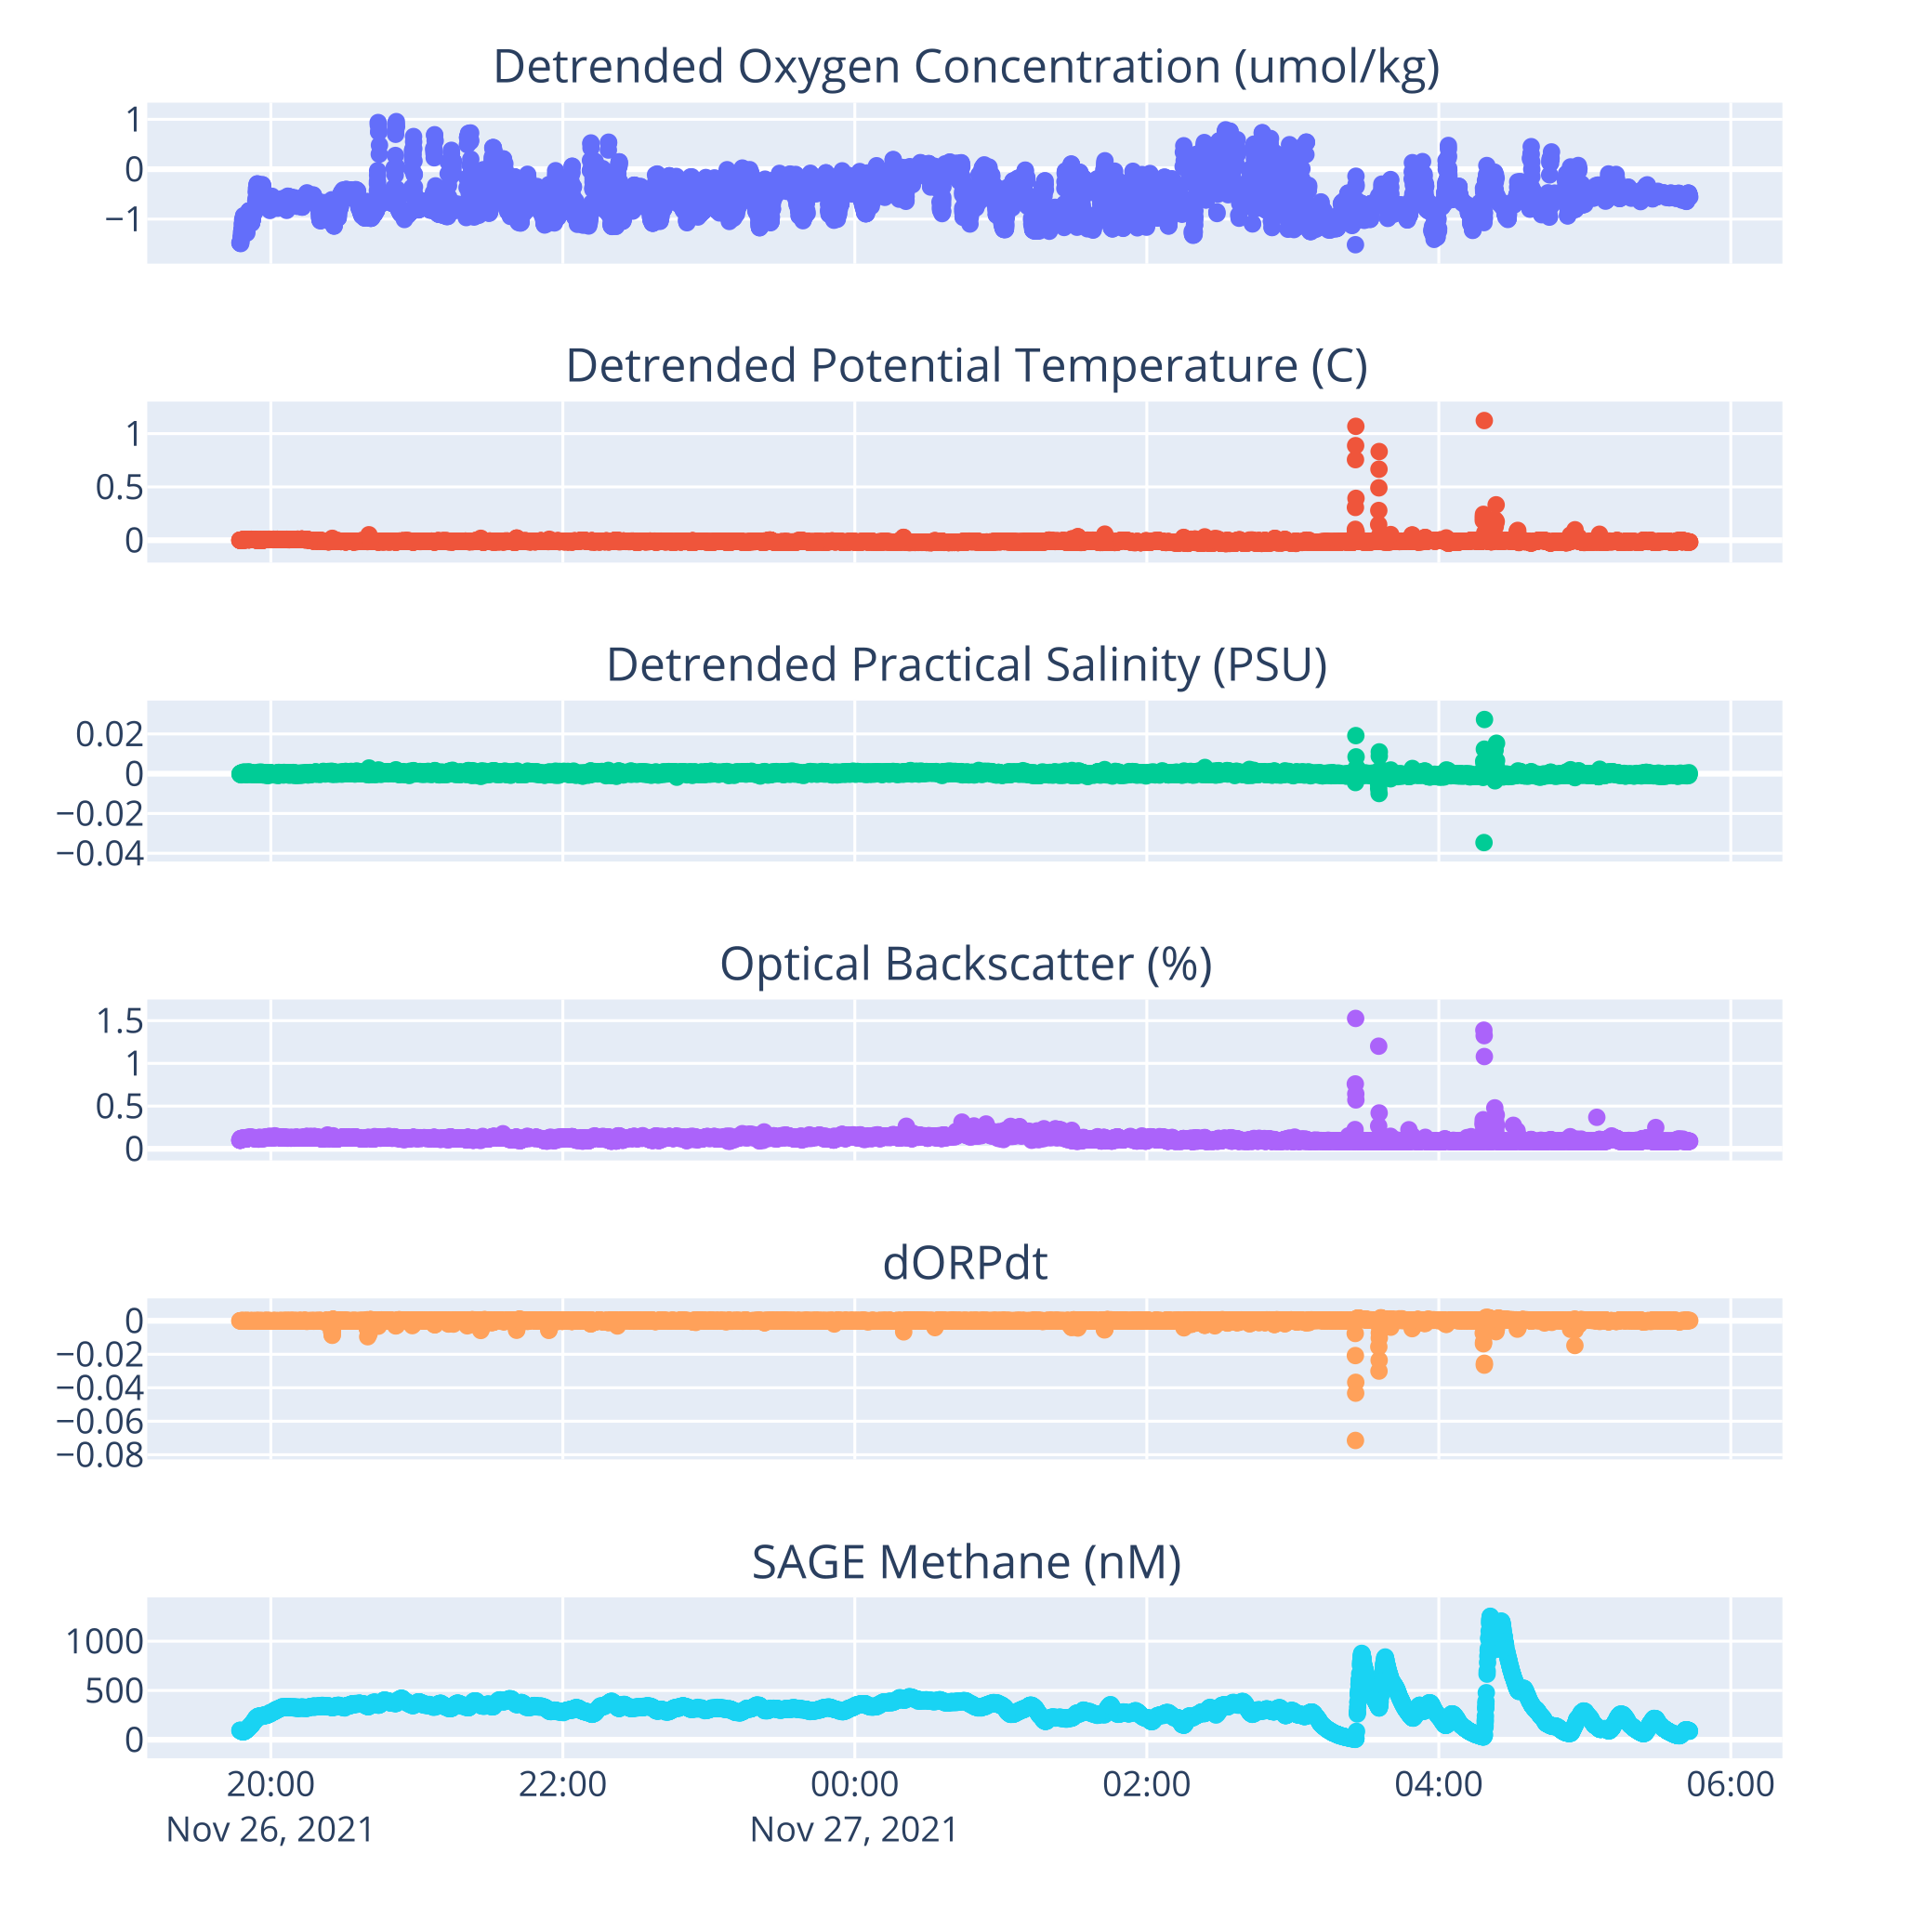
\includegraphics[width=0.45\columnwidth]{figures/binary_example_time.png}
    \hspace{.1in}
    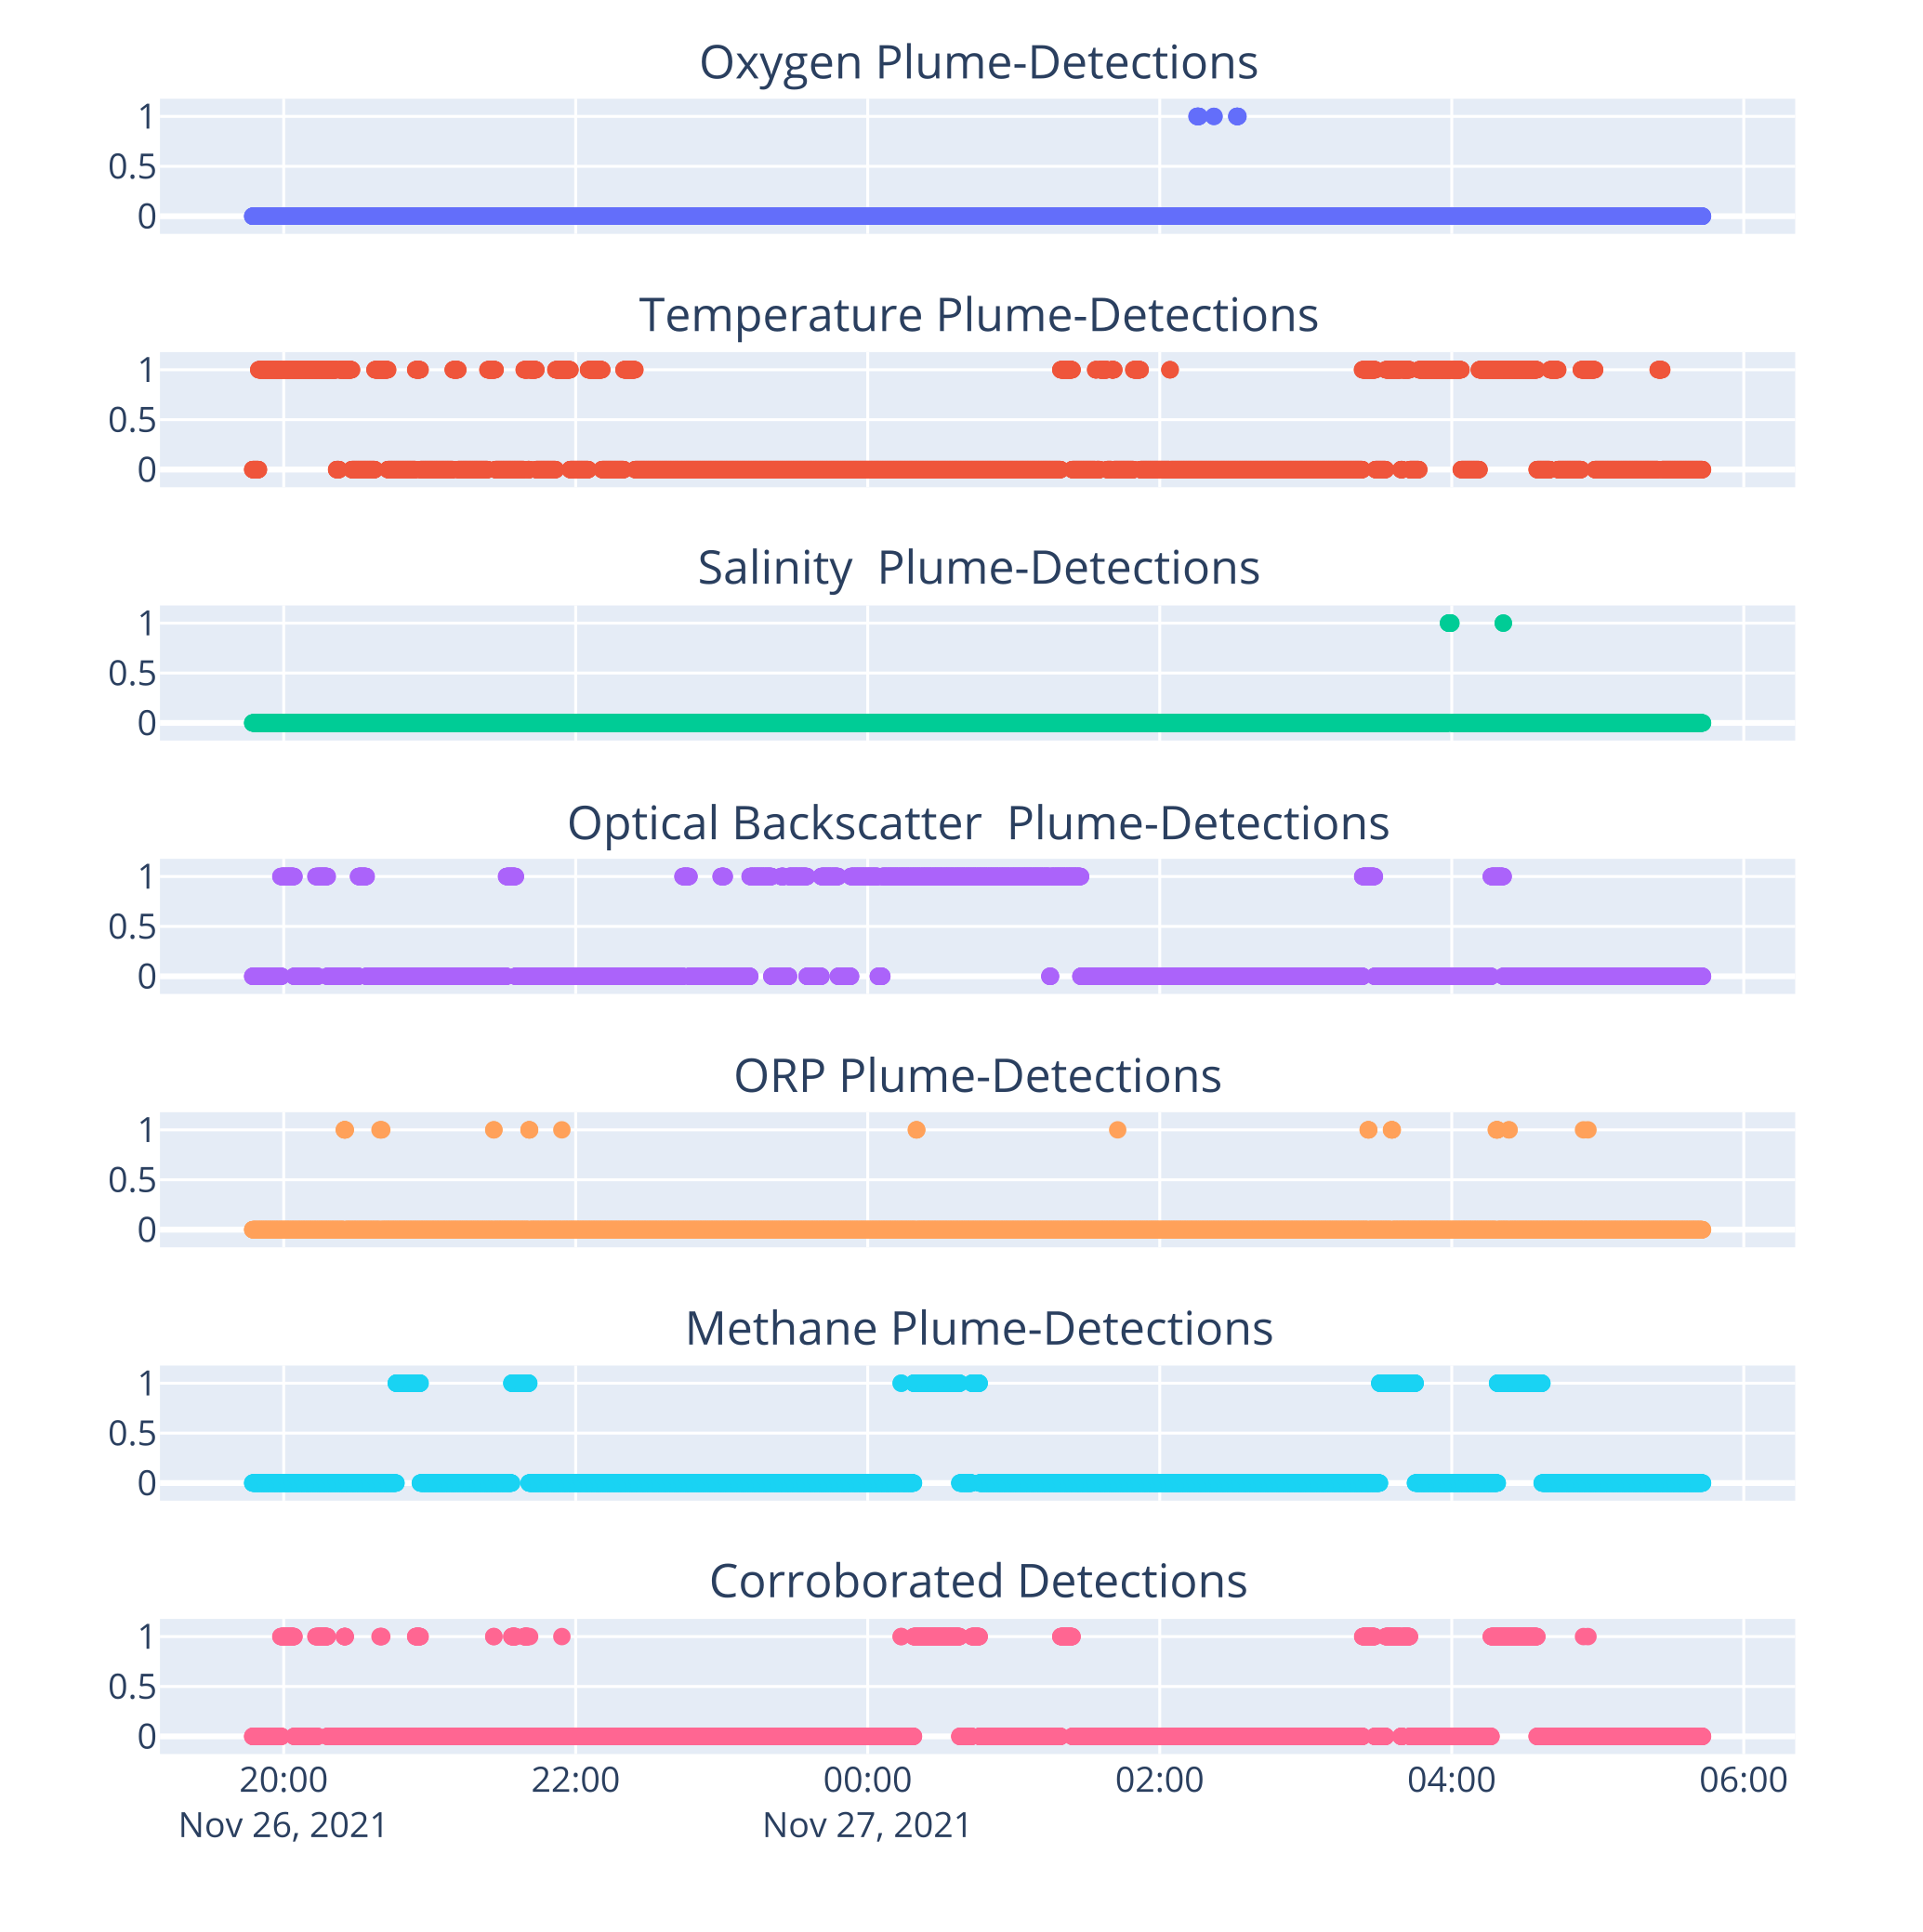
\includegraphics[width=0.45\columnwidth]{figures/binary_example_detections.png}
    \caption{Example time series (left) and associated detections (right) over the AUV \Sentry sensor suite. Oxygen, temperature, and salinity measurements are detrended using a linear transformation fit to depth vs. value plots. The time series demonstrates two types of plume detections. The first are ``obvious detections'' in which most sensors register strong anomalies (this happened twice toward the end of the deployment) and are most strongly associated with buoyant-stem derived fluids. The second are ``persistent-plume detections'' in which the robot traverses through water that is slightly more turbid, warm, or chemical-rich than background water over potentially long horizons (this happened early in the deployment and in the middle). Such detections are most strongly associated with neutrally-buoyant layers. The conservative corroboration detector successfully identifies both forms of plume water.}
    \label{fig:detection_example}
\end{figure}
 
The result of our sensor model is to convert multiple, time-stamped sensor observations $s_{t, i} \in \R, \, i = 1, \dots, S$ to a single, binary plume-detection $z_{p} \in \{0, 1\}$. These binary plume detections are then used to update our plume model and plan robot trajectories, as described in the following sections. The accuracy of this sensor model is currently uncharacterized, as there is no available ground truth in a field setting by which to verify the assigned classifications. Qualitatively, the classifications were reviewed by the science team and verified for their alignment with expert opinions on which label to assign.


%%%%%%%%%%%%%%%%%%%
% External Sensing 
%%%%%%%%%%%%%%%%%%
\subsection{External Sensing: Leveraging All Available Information}
\label{sec:external_current}
Outside of AUV \Sentry, several sensing packages were deployed during the research cruise which collect relevant information about the state of temporally evolving crossflow and ambient seawater properties. We leverage these external measurements within our \PHUMES instance in two ways: (1) setting default seawater constants of the target site, and (2) to learn the crossflow transition function $T_c$.

On the first point, measurements from a temperature and salinity sensor mounted to a ship-board rosette were used to define the density, temperature, and salinity stratification curve of the Guaymas Basin water column. The stratification curve is a function that describes the changes in density (or temperature and salinity) over depth in the ocean, and has implications for how a hydrothermal plume will interact with background seawater. The stratification function is used within the physically-informed layer of \PHUMES and treated as a constant throughout the expedition. This information could be equivalently extracted from sensors onboard \Sentry, but the available external sensing package was higher fidelity for the purpose of water column characterization. Moreover, as this information can be observed once and assumed to be effectively constant, it is convenient to incorporate this information outside of the sequential decision-making process.

On the second point, critically there was no ``current sensor'' on \Sentry available during our expedition that could be used to measure the \emph{in situ} current magnitude and heading during a deployment. While it may be possible to estimate $T_c$ solely from the binary observations of the plume, access to an external bottom-mounted tiltmeter on the seafloor during this expedition significantly relieved the burden of this inference process. We learn $T_c$ (or, more precisely, the function $h$ by which $T_c$ is defined) by fitting a Gaussian process (GP) with composite radial-basis-function and periodic kernel functions to point observations of crossflow magnitude and heading observed by the tiltmeter. Approximately 3 days of observations were available for training. Crossflow parameters $\x_c$ in $\Ss$ were set with the expected mean of the trained GP. Presently, a crossflow sensor is in development for \Sentry using existing acoustic technology onboard the robot; in such a configuration, the process of estimating $T_c$ would be dependent on robot actions and would be a less independent process to the plume-charting task.

% PHUMES
\subsection{\PHUMES: Physically-informed Probabilistic Forecasts}
\label{sec:phumes}
\PHUMES is a model class that can generate predictions of the distribution of a spatiotemporally evolving state from a history of sparse state-space observations. To quickly learn a predictive model of a spatiotemporal phenomenon, \PHUMES leverages access to analytical scientific simulators (when available) codified as systems of ordinary differential equations (ODEs). These simulators reduce the dimensionality of the inference problem from the full-state of the environmental phenomenon (e.g., a 4D volume in space and time with continuous phenomenon measurement) to the dimensionality of the initial conditions and parameters of the simulator (which can then be used to populate the full-state for planning purposes). The use of ODE systems, as opposed to high-fidelity numerical simulators using partial differential equations (PDEs) is intentional; the computational requirement of most PDE systems used to model environmental phenomenon at the scales studied during expeditionary missions are intractable. In contrast, ODE systems are less well-resolved, but summarize the structure of an evolving phenomenon in a useful way that can be enhanced by a generic probabilistic formulation wrapping the ODEs.

In the \PHUMES formulation for hydrothermal plume charting, we use a time-averaged model of plume evolution through a weakly stratified fluid under crossflow as described in \cite{tohidi2016highly} which we notate as function $f(\cdot, \cdot)$. The crossflow ``bends'' the buoyant stem of the plume, and reduces the effective rise height of the plume by introducing more mixing. Using a modified cylindrical coordinate system in which $s$ represents a point along the axis described by the plume centerline and $\theta$ describes the vertical angle from the base of the plume, our \PHUMES simulator takes the form:

\begin{equation}
    \frac{dQ}{ds} = Q\sqrt{\frac{2(1+\lambda^2)}{M\lambda}}(\alpha|\frac{M}{Q} - U_a\cos\theta| + \beta|U_a\sin\theta|)
\end{equation}
\begin{equation}
    \frac{dM}{ds} - U_a\cos\theta\frac{dQ}{ds} = \frac{FQ}{M}\sin\theta 
\end{equation}
\begin{equation}
    U\sin\theta\frac{dQ}{ds} + M\frac{d\theta}{ds} = \frac{FQ}{M}\cos\theta
\end{equation}
\begin{equation}
    \frac{dF}{ds} = -QN^2\sin\theta
\end{equation}
\begin{equation}
    x_a = \int_0^s\cos\theta ds
\end{equation}
\begin{equation}
    h_a = \int_0^s \sin\theta ds
\end{equation}

where $U_a = U_a(z)$ is the ambient crossflow velocity, $Q = Q(s,\theta)$ represents the plume specific volume flux, $M = M(s, \theta)$ is the specific momentum flux, $F = F(s, \theta)$ is specific buoyancy flux, $N$ is the Brunt-V\"ais\"al\"a frequency, $\lambda$ is the ratio of the minor and major axis that define the plume cross-sectional ellipse, $x_a$ and $h_a$ represents the Cartesian transform of $s$ and $\theta$ within the plume's frame of reference, and $\alpha$ and $\beta$ are vertical and horizontal entrainment coefficients. To convert abstract notions of buoyancy and momentum flux to directly observable/meaningful vent characteristics like vent area or fluid exit velocity, we can use the following relationships:

\begin{equation}
    Q_0 = \lambda u_0 \frac{A_0}{\pi}
\end{equation}
\begin{equation}
    M_0 = Q_0 u_0
\end{equation}
\begin{equation}
    F_0 = g10^{-4}(T-T_0)Q_0
\end{equation}

\noindent where $A_0$ is the vent area, $u_0$ is the initial fluid velocity leaving the vent, $T$ is the temperature of fluid at the vent, and $T_0$ is the temperature of ambient seawater at the depth of the vent (note that temperature is the dominant component of density, $\rho$, for deep-sea hydrothermal plumes). Indeed, temperature, area, and exit velocity compose a sufficient set of parameters for representing the initial conditions of any particular plume and plume envelope calculation; these quantities, in addition to the mixing coefficients, form our set of $\x_p$ in $\Ss$ in the plume-charting POMDP. $U_a$ and the global heading of the crossflow, $\Theta_a$ (not directly modeled in these equations, but can be trivially applied to $x_a$ and $x_h$ to convert plume-reference coordinates to global coordinates), form the parameters in $\x_c$ in $\Ss$.

With the simulator defined, we can now pose a specific inference problem: from observations of plume or background waters, what are the generating initial conditions (vent area, vent fluid temperature, vent fluid exit velocity) and seawater properties (horizontal mixing coefficient, vertical mixing coefficient, global current heading (at a moment in time), and global current magnitude (at a moment in time))? This explicitly allows us to place probability distributions over $\x_p$ and $\x_c$, over which we initially place an uninformative prior, $\Pi(\x_p)$ and $\Pi(\x_c)$ and aim to learn the posterior distributions $\Pi(\x_p | \Zz)$ and $\Pi(\x_c | \Zz)$ \footnote{We effectively separate inference over $\x_p$ and $\x_c$ given the observation model available; indeed we assume that observations of crossflow can be treated as independent of observations of plume detections. This is strongly supported in the practical deployment of \Sentry, when an external sensor was necessary to observe crossflow. If instead the sensors were co-located on \Sentry, inference over the joint posterior $\Pi(\x_p, \x_c | \Zz)$ could be done instead.}.

\begin{figure}[h!]
    \centering
    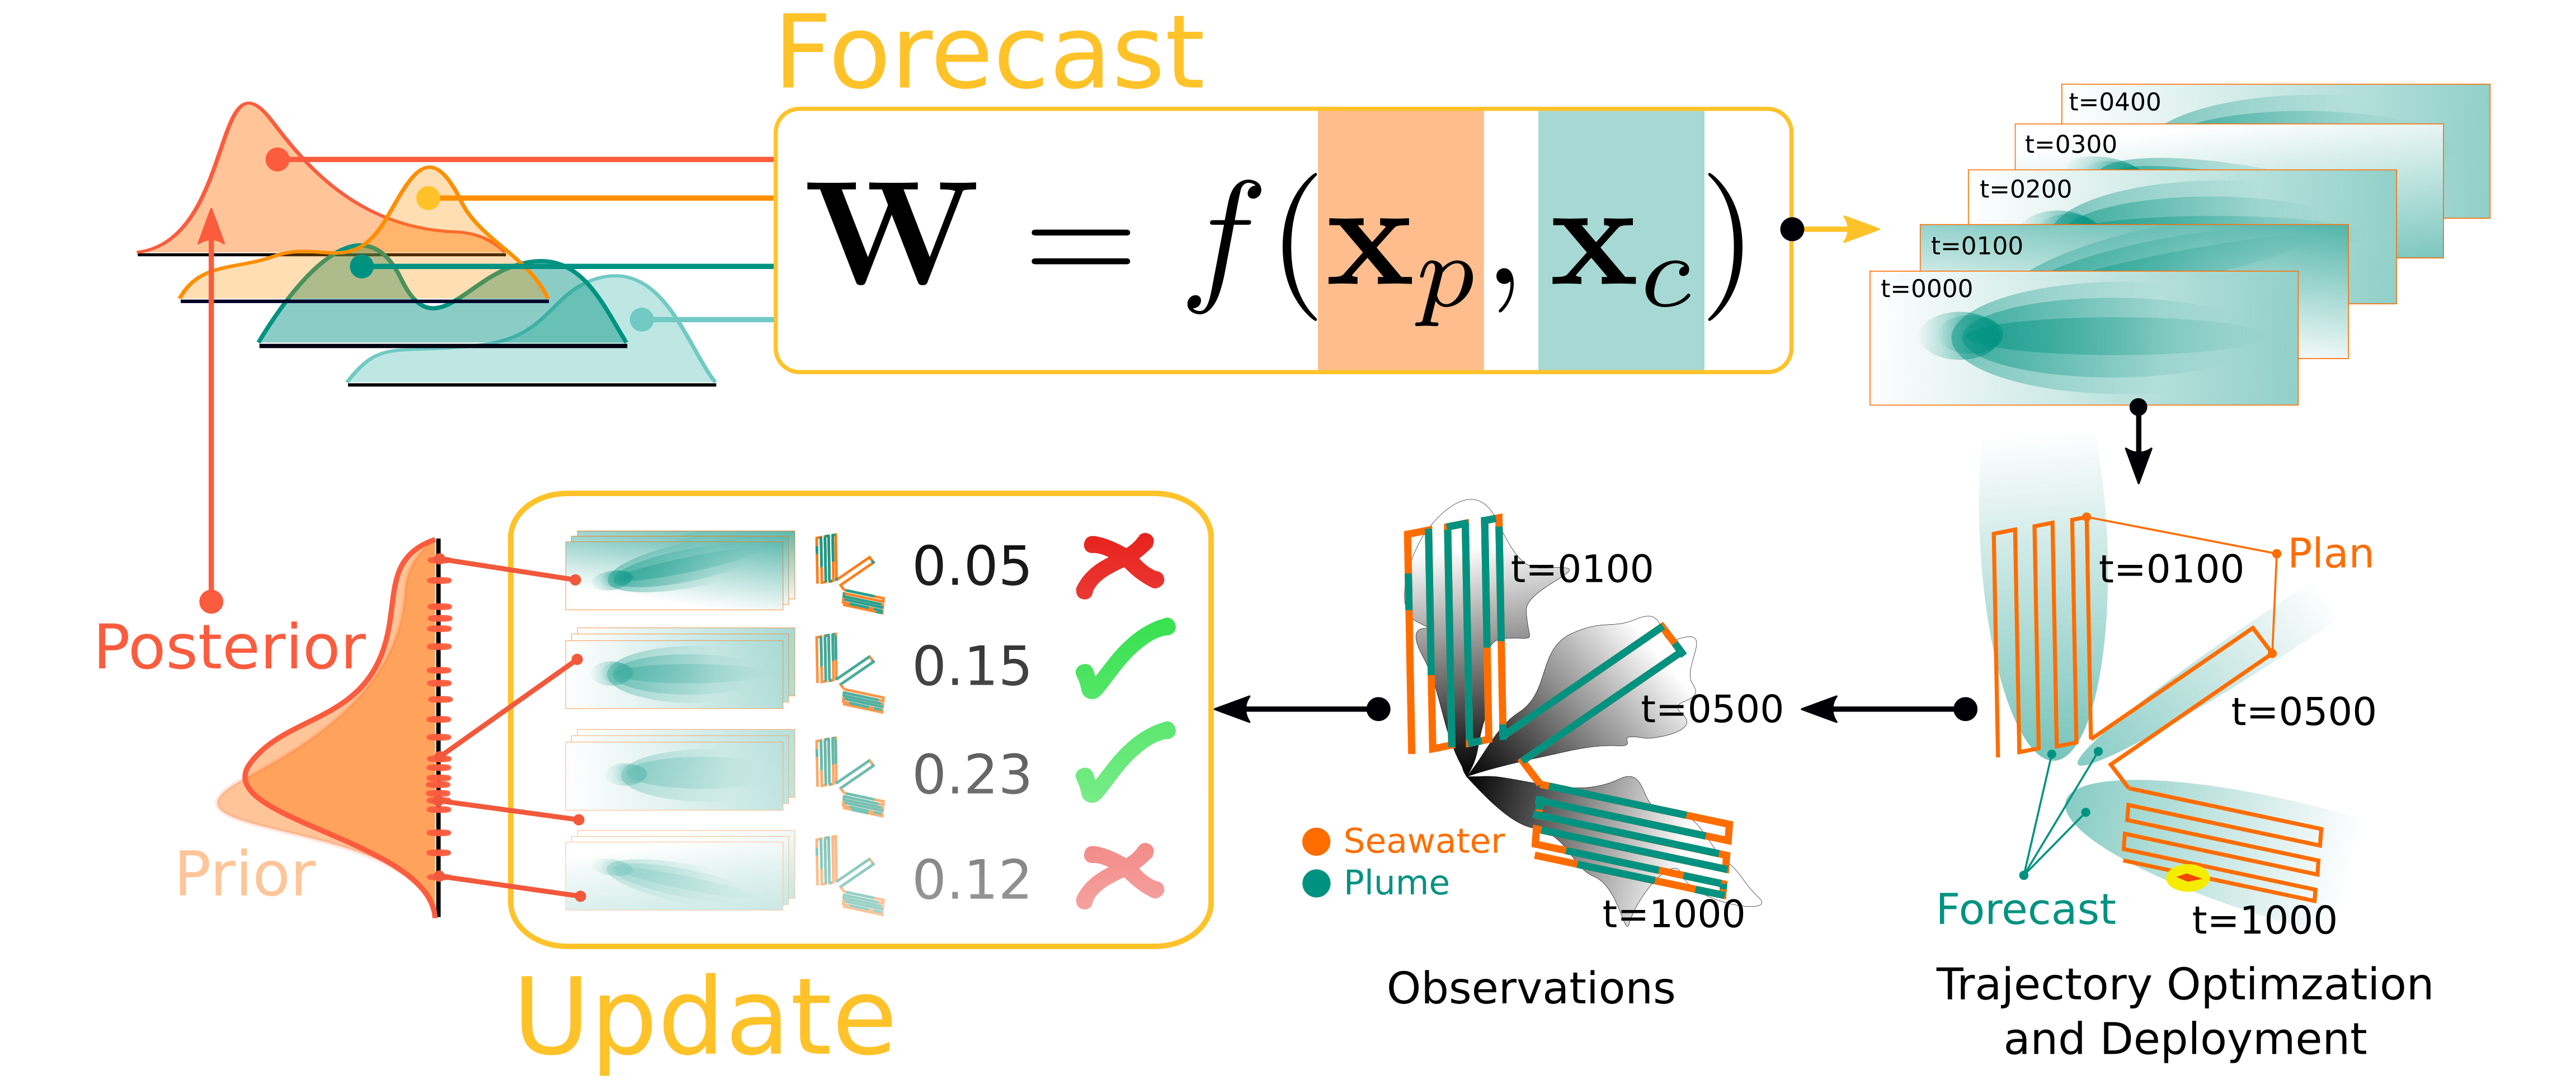
\includegraphics[width=1\columnwidth]{figures/phumes_diagram.png}
    \caption{\PHUMES: \phumes; a model class for forecasting spatiotemporal distribution evolution trained on partial observations. \PHUMES generates forecasts by leveraging an embedded analytical model $f(\cdot, \cdot)$ that approximates the physics-driven evolution of a target distribution. This model is seeded with many samples from distributions placed over initial conditions, physical parameters, or temporal functions (such as $\x_p$ and $\x_c$ here). The composite result of this process is a forecast $\mathbf{W}$ that consists of a mean and variance of phenomenon occupancy in a 3D volume over snapshots of time. This forecast is provided to a trajectory optimizer which sets a deployment trajectory that is executed by a robot. The deployment generates a series of observations, which are then used to update the distributions of the generating distributions via an MCMC procedure which compares the gathered observations with the simulated observations of samples from the generating distributions. The resulting posterior update over the generating distributions is then used for the next planning iteration.}
    \label{fig:phumes}
\end{figure}

\PHUMES consists of two key phases: forecasting (forward simulation) and updating (inverse problem) (\cref{fig:phumes}). In the forecasting step, samples from the distributions of the initial conditions and seawater properties seed the simulator which is solved many times to create a set of plume-envelope samples in the full state space of the target phenomenon (and trajectory optimizer). Time is discretized over domain-specific key points, and any parameters reliant on time are sampled at those discrete points. The set of composite samples at each time is a ``forecast'' that is essentially a series of ``snapshots'' of the phenomenon. Precisely, \PHUMES generates a time-indexed $t \in \mathbb{T}$ composite estimate of the distribution of plume fluid in a 3D volume $\overbar{\mathbf{W}}$ by forward simulating time-dependent $M$ samples of the states $x_{p,t}^{(m)} \sim \Pi(\x_p(t))$ and $x_{c,t}^{(m)} \sim \Pi(\x_c(t))$ through the plume simulator $f(\cdot, \cdot)$:

\begin{equation}
    \overbar{\mathbf{W}_t} = \frac{1}{M}\sum_{m=1}^{M} f(x_{p,t}^{(m)}, x_{c,t}^{(m)}) \hspace{1cm} \forall t \in \mathbb{T}.
\end{equation}

The complete forecast $\overbar{\mathbf{W}}$ is then used by a trajectory optimizer to approximate the reward function $R([\x_p, \x_c, \x_r]^T, a) = \indic{\texttt{in\_plume}(\x_p, \x_c, \x_r, a)} \approx \indic{\texttt{in\_plume}(\overbar{\mathbf{W}}, a)}$. Equivalently, $\mathbf{W}$ is the robot's belief $b$. The variance of the forecast $\mathbf{S}^2_W$ can be similarly computed, depending on the requirements of the reward function. 

After the trajectory optimizer yields a plan, \Sentry is deployed. For a single deployment, upwards of 20,000 observations may be available (each deployment is a minimum of 6 hrs in duration, up to 24 hrs, and sensor measurements are logged at 1 Hz). Using the filter described in \cref{sec:sensor_models}, AUV \Sentry provides observations of binary plume detections. Other sensors of opportunity described in \cref{sec:external_current} provide continuous crossflow magnitude and heading observations. These observations are collated into the sensor model $\Zz$.

At the update step of \PHUMES, the distributions over $\x_p$ and $\x_c$ are updated from observations $\Zz$. To find $\Pi(\x_c|\Zz)$ we use GP models for crossflow magnitude and heading as described in \cref{sec:external_current}. A bulk, closed-form analytic update is made to the GP kernel parameters following typical procedures \cite{Rasmussen2004}. For $\Pi(\x_p | \Zz)$, we use a random-walk Metropolis-Hastings MCMC method \cite{metropolis1953equation} to perform the update. Simulations of deployments are generated by solutions to the numerical model seeded with samples from $\x_p$ and $\x_c$. The output of the simulations is directly compared via a likelihood model with the observations binary observations of plume waters collected by \Sentry. In practice, the likelihood model uses a false positive rate (the observation is a 1, and the simulation is a 0) and false negative rate (the observation is a 0, and the simulation is a 1) established in consultation with instrument experts on the science team; they are set to 0.1 and 0.3, respectively. With the likelihood model applied, samples of $\x_p$ are then stochastically accepted or rejected. As this inference method is a chaining procedure, the samples of $\x_p$ selected in this procedure are informed by the last, and the cumulative distribution of accepted samples is guaranteed to converge to the true underlying distribution for each of the elements in $\x_p$. The posterior distribution $\Pi(\x_p | Z)$ is set as the new sampling distribution for the next forecast to be generated.

\subsection{Trajectory Optimization for Path Planning with Fixed Primitives}
\label{sec:to}
\td{some edits are necessary to this section based on feedback; particularly separating the definition of the optimization from the implementation details} 

To solve the plume-charting sequential decision-making problem, we begin with the POMDP value function \cref{eq:value} and introduce the model defined in \cref{sec:problem}:
\begin{align}
     V_h^{*}(b) &=  \max_{\{\theta_1, \dots, \theta_n, n \mid \theta_i \in \Theta, n \in \Z^+\}} \mathbb{E}_{[\x_{p}, \x_{c}, \x_{r}]^\top \sim b}[R([\x_{p}, \x_{c}, \x_{r}]^\top, \{\theta_1, \dots, \theta_n\})] \hspace{0.6cm} h \in [0, H-1],
    \label{eq:approx_value}
\end{align}
where $\theta \in \Theta$ parameterizes individual trajectory primitives in a length-$n$ sequence of chained trajectories and $b$ is the planner's belief about the state of the plume, currents, and robot, and the discount factor $\gamma$ has been set to zero to encode our single-dive planning approximation. Solving \cref{eq:approx_value} still involves the challenging optimization of $n$ trajectories and the joint optimization of all $n$ trajectories into a chain. To simplify the planning problem, given the constraints of real-world robotic deployments, we assume that the number of chained trajectories is given, i.e., $n=N$, and that each trajectory can be optimized independently. This results in the following approximation:
\begin{align}
     V_h^{*}(b) &\approx  \max_{\theta_1 \in \Theta} \dots \max_{\theta_N\in \Theta} \mathbb{E}_{[\x_{p}, \x_{c}, \x_{r}]^\top \sim b}[R([\x_{p}, \x_{c}, \x_{r}]^\top, \{\theta_1, \dots, \theta_N\})] \hspace{0.6cm} h \in [0, H-1].
    \label{eq:approx2_value}
\end{align}

We solve \cref{eq:approx2_value}, which defines multiple, independent, non-convex, constrained optimization problems, using the trust-constrained method in the \texttt{scipy} optimization library for a fixed number of iterations \cite{conn2000trust}. To evaluate the reward function $R([\x_{p}, \x_{c}, \x_{r}]^\top, \{\theta_1, \dots, \theta_N\})$, we define a trajectory sampler operator $\Gen: \Theta \to \R^{3 \times k}$ that takes a trajectory parameter vector as input and produces a set of locations in $\R^3$ that will be sampled when the robot executes the trajectory, where $k$ is the number of sampled points. These sample points can then be compared with the plume forecast $\mathbf{W}$ produced by \PHUMES to count the number of sample points that are contained within the inferred plume.

In practice, we choose our trajectory class to be a lawnmower trajectory, which were parameterized by a vector $\theta$ that determines the origin, orientation, height, width, and resolution of the lawnmower. The trajectory sampler $\Gen$ produces the lawnmower specified by $\theta$ and then subsamples uniformly along its length. We defined the set $\Theta$ to enforce that the lawnmower trajectories are contained within a pre-defined, rectangular safe region and that each lawnmower obeys a time-based budget constraint.


\subsection{At Sea Operations}
When performing field operations on the research vessel with AUV \emph{Sentry}, we used \PHORTEX to enable deployment-by-deployment autonomy that could iteratively improve robot performance with each deployment (\cref{fig:at_sea_ops}). Functionally, the trajectories planned with \PHORTEX were provided to the \Sentry engineering team for extensive safety validation prior to each deployment. If approved by the \Sentry team, the chief scientist, and captain of the vessel, the trajectories were downloaded into the \Sentry mission planning software as static waypoints. This confirmation process required a lead time of approximately 6 hrs before a given deployment time, and approximately 12 hrs were available between deployments to mechanically service \Sentry and recharge batteries. The ability of \PHORTEX to produce viable trajectories from data within the first 6 hrs that \Sentry was on-deck following a recovery was critical for keeping this strict timeline. Given the long lead time between trajectory design and \Sentry deployment, there were many opportunities for the time of a deployment to change due to developments in weather, other science/technology priorities, a critical personnel was occupied, etc. To be robust to these changes, we provided deployment plans that started several hours before and several hours after a given deployment time, and the \Sentry team truncated the plan at the appropriate point once a deployment time was known with certainty.

\begin{figure}[h!]
    \centering
    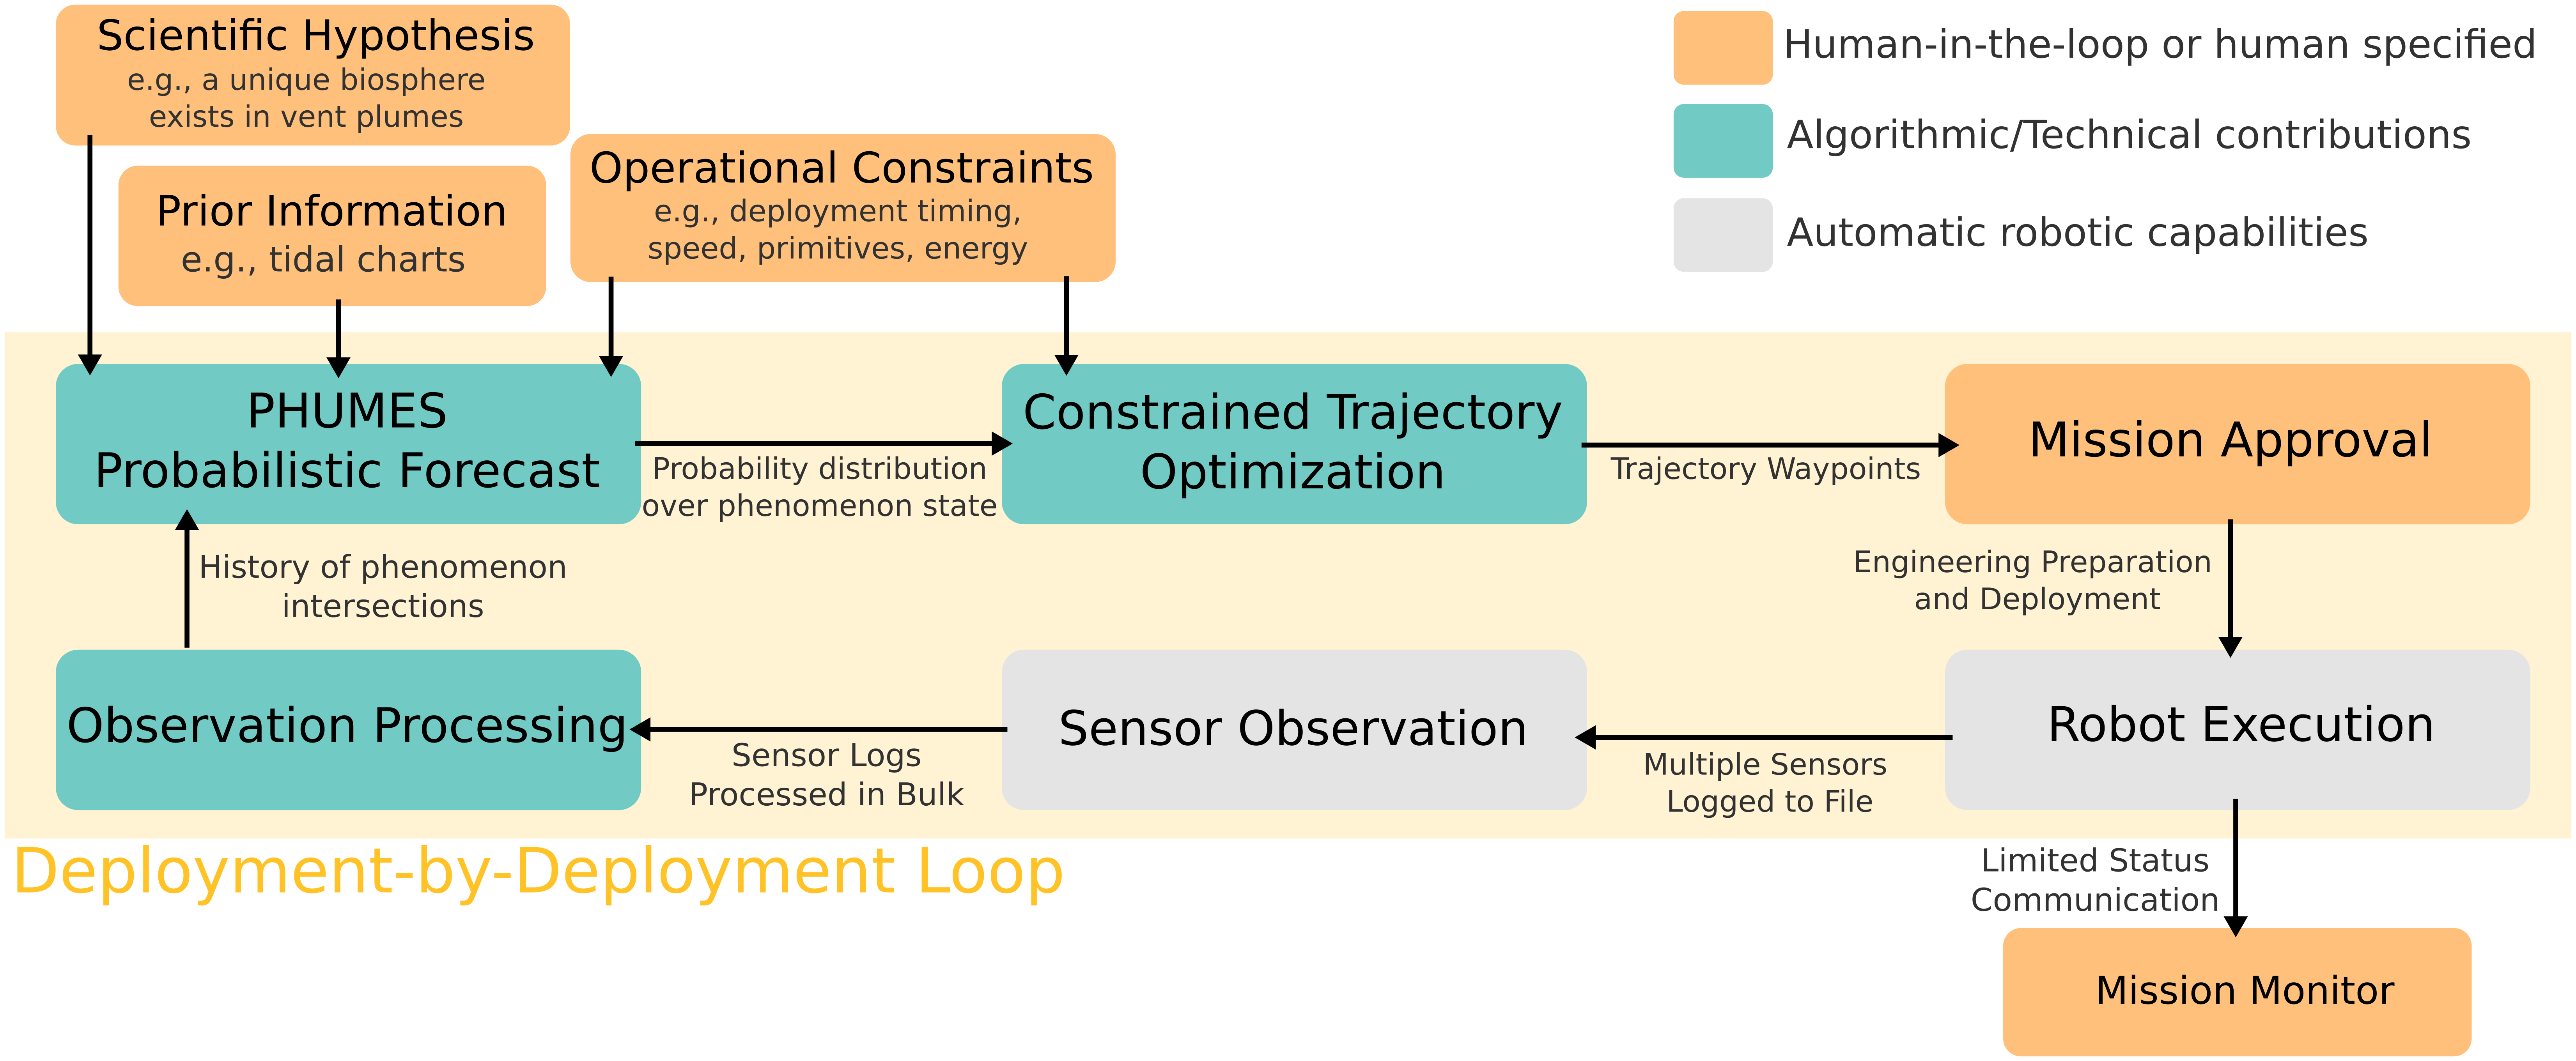
\includegraphics[width=1\columnwidth]{figures/deployment_loop.png}
    \caption{The at-sea operations implementation of \PHORTEX. Integration of scientific knowledge, prior information, auxiliary sensor information, and operational constraints was done at the initialization of the \PHORTEX deployment-by-deployment loop. Every trajectory generated by \PHORTEX was checked by AUV \Sentry engineers and the science team before execution. \Sentry status was monitored with an external acoustic tracking system that monitored vehicle location, power, and performance while in acoustic range of the ship. Upon returning to deck, all science sensor observations were downloaded in bulk from the vehicle, and then ingested via our \PHORTEX system.}
    \label{fig:at_sea_ops}
\end{figure}



\section{Field Deployment: Charting Deep-Sea Hydrothermal Plumes}
\label{sec:field_results}

In November 2021, a research cruise aboard the Research Vessel (R/V) \emph{Roger Revelle} was conducted to the Northern Guaymas Basin in the Gulf of California to study a recently discovered hydrothermal ridge \cite{soule2018exploration, geilert2018formation}. The research cruise had several objectives: test novel \emph{in situ} instruments to measure dissolved methane, test novel \emph{in situ} instruments to measure the carbonate cycle, map the heat distribution in shallow sediments above hydrothermal sills, collect specimens of tubeworms, and collect biological samples of microbiota in hydrothermal plume-fluids for \emph{ex situ} analysis to re-construct the structure of a plume microbiome. It is typical that research cruises have several science teams working together under an appointed chief scientist to maximize the use of ship assets while at sea. To assist in operations, AUV \Sentry, remotely-operated vehicle (ROV) \emph{JASON}, and standard oceanographic acoustic and profiling equipment were available. The deployment of \PHORTEX on the cruise for \Sentry operations was coupled with objectives to test \emph{in situ} instruments and collect microbiota samples. For both of these tasks, charting different regions within a plume structure was important to test the limits of the novel instruments and collect microbiota samples from a diversity of plume-conditions.


\subsection{Site Description and General Conditions}
The main site for the study conducted by AUV \Sentry using \PHORTEX is a hydrothermal ridge located in the northern Guaymas Basin, approximately \SI{1850}{\meter} underwater and at the edge of an additionally \SI{300}{\meter} deeper graben (a valley with steep sides) (\cref{fig:site}). The ridge is approximately \SI{600}{\meter} long and features several tall sulfide structures 45-\SI{75}{\meter} in height with active smoking along their bodies. A smoking ``chimney'' at the northernmost point of the ridge was targeted for plume-charting. Composed of a cluster of tens of small orifices ($<$\SI{0.1}{\meter} diameter) creating an approximately \SI{1.5}{\meter} diameter chimney base, the fluid produced was thick with particulate matter, \SI{340}{\celsius} at the source, ventilated rapidly at approximately \SI{0.7}{\meter\per\second} (as measured by video equipment), and rich in dissolved methane. In contrast, the ambient seawater was methane-poor, considerably less turbid, and cold at \SI{4}{\celsius}. Vent characteristics were measured by ROV \emph{JASON} carrying specialized sensing equipment, and we use these measurements as a means of seeding and measuring the performance of \PHUMES within \PHORTEX.

\begin{figure}[h!]
    \centering
    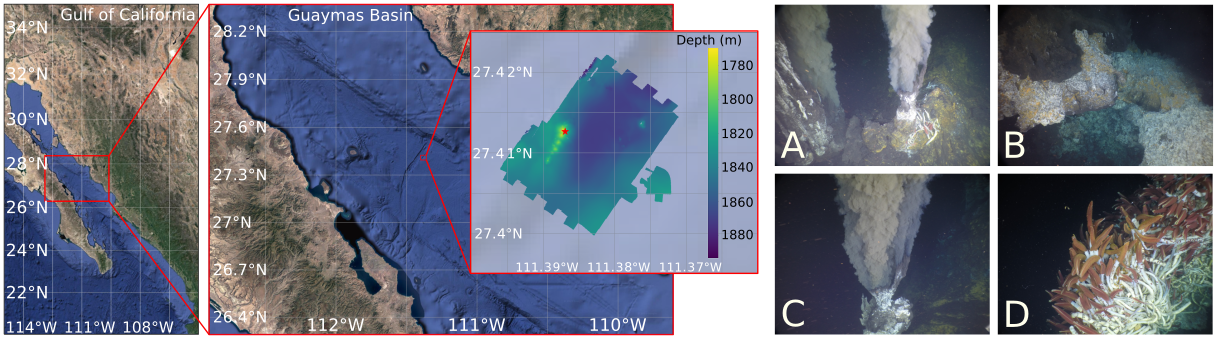
\includegraphics[width=\columnwidth]{figures/site_summary.png}
    \caption{Study site in the Guaymas Basin, Gulf of California. The inset map is bathymetric data collected by AUV \Sentry during this expedition and shows the approximately \SI{600}{\meter} long ridge in yellow. The red star marks the chimney that was of particular study in this article. Pictures A-D show imagery from the ridge and chimney site. A-C show various forms of plume-producing vents located at the chimney and D shows an example of the macrofauna covering the structures along the ridge.}
    \label{fig:site}
\end{figure}

As vent fluids rise and form a plume at this site, the ambient water is mixed (entrained) at an unknown rate. The presence of advective crossflow, reaching magnitudes up to \SI{0.1}{\meter\per\second}, was obvious from images of the bending plume stem at the vent sites (and was measured by the bottom-mounted tiltmeters deployed during the expedition). The magnitude and heading of the crossflow appeared to be semi-cyclic, following a pattern (albeit time-delayed) established by tidal charts produced by Centro de Investigaci\'on Cient\'ifica y de Educaci\'on Superior de Ensenada (CISESE) for the time period of the expedition\footnote{Charts available from: \url{www.predmar.cicese.mx/calendarios}}. Local bathymetric and other physical effects on crossflow were also qualitatively observed. Under these conditions, plume expressions could be transported several hundred meters from a known source, and would be expected to rise over \SI{200}{\meter} in the water column. In scientific work following this expedition, plume fluids were identified from collected observations over \SI{7}{\kilo\meter} away from known venting sites [IN PREP]. 


\subsection{Overview of Sea Trials with AUV \Sentry}
Four deployments as part of the \PHORTEX study were made with AUV \Sentry, and represent a planning ``spectrum'' from fully human-designed surveys to fully \PHORTEX designed. We label the four deployments as follows:
\begin{itemize}
    \item \textbf{Dive H-Multi}: human designed, multi-task survey. This was the first deployment of \Sentry and the survey was designed to both attempt to find plume fluids and to bathymetrically map the local basin area (the map of which would be used as part of the safety check protocol for future deployments). This dive is representative of a standard ``nested'' strategy, in which progressively more targeted (finer resolution) surveys are used to study areas that might be of interest. The deployment lasted 21.3 hrs and collected 76,604 observations total.
    \item \textbf{Dive H-Plume}: human designed, plume-charting survey. This was the second deployment of \Sentry and the survey was hand-designed by the science party onboard the vessel to find and sample plume fluids. The science party had access to the performance of \Sentry in Dive H-Multi. The strategy was to sweep the basin above areas with known hydrothermal vents, and fly out into the basin in the direction that the plume fluids would be expected to advect. The deployment lasted 21 hrs and collected 75,430 observations total.
    \item \textbf{Dive HP-Plume}: hybrid human and \PHORTEX plume-charting survey. This was the third deployment of \Sentry and the survey consisted of trajectories designed by \PHORTEX trained by observations collected in Dive H-Multi. Two of the trajectory primitives designed by \PHORTEX were replaced by ``naive'' lawnmowers placed over the known vent at two different times in the deployment. The deployment lasted 22.2 hrs and collected 79,792 observations total. Of these, 8.2 hrs and 29438 observations were collected via the naive strategy.
    \item \textbf{Dive P-Plume}: \PHORTEX plume-charting survey. This was the fourth and last deployment of \Sentry. The survey was fully designed by \PHORTEX using observations from Dive H-Multi. The deployment lasted 9.9 hrs and collected 35,755 observations total. This deployment is notably much shorter than the other deployments due to increasing time constraints as the expedition was coming to a close. This deployment also used \Sentry in a ``depth-hold'' mode; whereas in all other dives \Sentry's depth followed the basin terrain, in this experiment the robot held an absolute depth.
\end{itemize}

\subsection{Experimental Results}
We look at several key metrics for each deployment: proportion of positive plume observations, utilization of spatial extent, and utilization of temporal window. The first metric, proportion of positive plume observations, is simply the number of observations collected in a dive that were classified as in-plume by the binary psuedo-sensor we describe in \cref{sec:sensor_models}. The second metric attempts to show how effective the design of the survey was spatially by first showing the absolute range that positive detections were made as a measure of distance from the chimney vent location and second showing how that range fit with the overall design of the survey. For example, if detections were made up to 300 m away from the vent, but the robot traveled up to 1 km away, then the survey spent too much time outside of the detectable plume region and would not be as effective as a survey that only traveled 200 m away but stayed well within the detectable plume range. Finally, the last metric is a measure of how effective the survey was at \emph{staying} or \emph{revisiting} a plume over time. Given the duration of these missions, it is important to use the entire mission window for the task at hand; moreover temporally ``diverse'' observations are of scientific interest generally. We report the dive hours with at least 10\% or more positive detections.

A summary of these metrics for each dive is provided in \cref{tab:field_results} and visualized in \cref{fig:field_results}. In general, we see that \PHORTEX performs as least as well as the human-designed surveys in terms of total number of samples collected, while improving spatial utilization (both with respect to effective utilization of the entire explored range, and in terms of increasing the effective detection range over naive trajectories placed ``on top'' of the vent). Absolute temporal utilization is similar to human surveys, however the distribution of detections within the temporal utilization windows is potentially improved---for human surveys, detections tend to be ``bunched'' to either the first half (as in H-Plume) or second half (as in H-Multi). Anecdotally, in HP-Plume, the two human-designed surveys occur in hours 5-8 and 20-23. While there were detections in both of these windows, over 90\% of total positive detections by these trajectories were collected only in the window from hours 20-23; in contrast the proportion of positive samples in the \PHORTEX designed trajectories in HP-Plume were more uniformly distributed in time (approximately 40\% collection in each window). 

\begin{table}[h!]
    \centering
    \begin{tabular}{c|c|c|c|c|c}
        Dive & Duration & Total Obs. & Prop. In-Plume & Spatial Util. & Temporal Util.  \\
        \hline
        H-Multi & 21.3 hrs & 76,604 & 22.3\% & \SI{300}{\meter} (19\%) & 9-17,20-21 (52\%) \\
        H-Plume & 21 hrs & 75,430 & 10.9\% & \SI{900}{\meter} (64\%) & 2,5-8,10-11,15-16 (43\%) \\
        \hline
        HP-Plume & 22.2 hrs & 79,792 & 41.8\% & \SI{600}{\meter} (100\%) & 1-3,5,7,11-23 (81\%) \\
        HP-Plume (H) & 8.2 hrs & 29,438 & 42.3\% & \SI{250}{\meter} (100\%) & 5,7,20-23 (75\%) \\
        HP-Plume (P) & 14 hrs & 50,354 & 41.5\% & \SI{600}{\meter} (100\%) &  1-3,11-20 (93\%)\\
        \hline
        P-Plume & 9.9 hrs & 35,755 & 12.8\% & \SI{450}{\meter} (100\%) & 1,5,8,9 (40\%)
    \end{tabular}
    \caption{Per-deployment statistics for field trials of \PHORTEX. The deployment HP-Plume is broken further into human designed (H) and \PHORTEX designed (P) portions for direct comparison.}
    \label{tab:field_results}
\end{table}

\begin{figure}[h!]
    \centering
    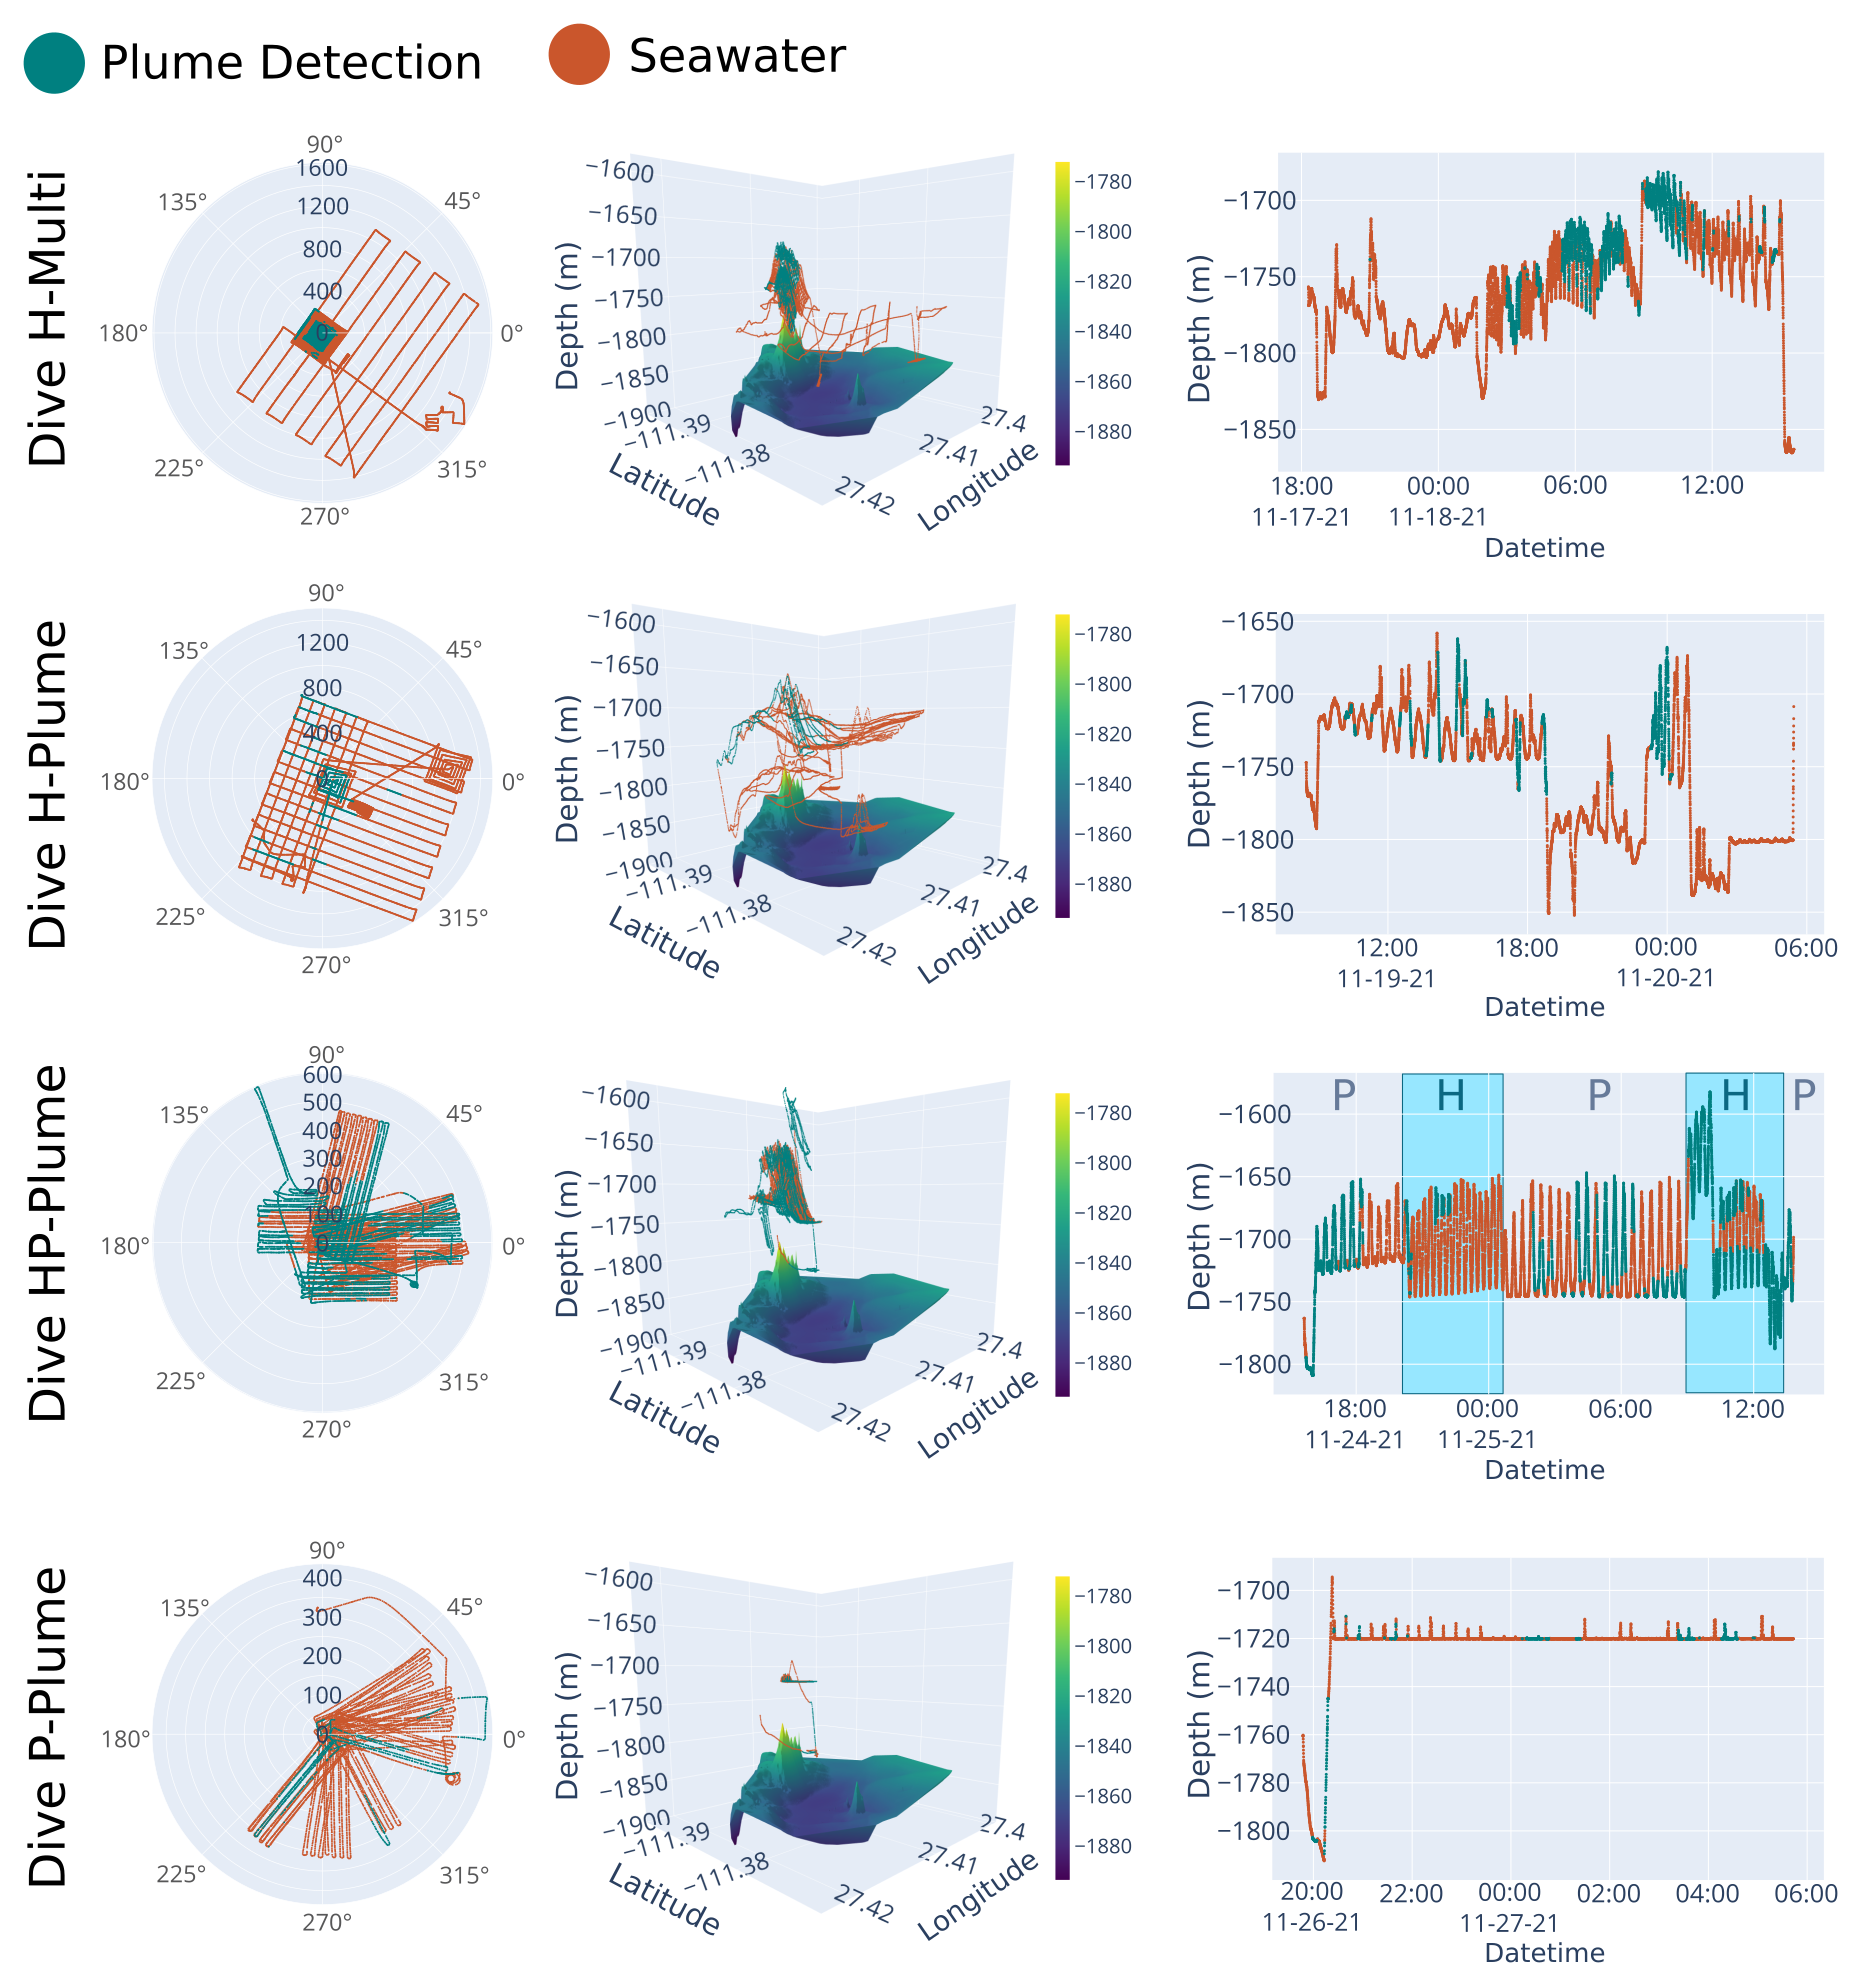
\includegraphics[width=1\columnwidth]{figures/detections_data.png}
    \caption{The four field dives of AUV \Sentry. All data is plotted according to its detection identity (in-plume or seawater). The first column shows a top-view of the dive trajectories in polar coordinates, in which angle and radius is computed relative to the chimney coordinate of the vent of study. In the center column, the 3D path of the vehicle over the rendered bathymetric terrain is provided. All but Dive P-Plume were dives conducted in altitude-hold mode with \Sentry, and so the trajectories show obvious changes in elevation; in contrast Dive P-Plume was held in depth-hold mode, so most observations are gathered within a depth-plane. The final column shows a time series versus depth of the detections collected. In Dive HP-Plume the portions of the dive that were human-designed and \PHORTEX-designed are labeled with H and P, respectively. As can be seen in the Dive HP-Plume time series, the two human-designed trajectories have significantly different performance, despite being in locally similar regions of the spatial domain. }
    \label{fig:field_results}
\end{figure}

In this field deployment it is obvious that \PHORTEX could be a useful tool for plume-charting. The performance of trajectories designed with \PHORTEX are comparable to those designed by humans with key possible improvements in spatial and temporal utilization. Moreover, the automated nature of \PHORTEX operationally alleviates significant decision-making burden on a science team and the trajectory-design burden on the \Sentry team; the ability to ingest data from external sensors and previous \Sentry missions, and produce trajectories that can be seamlessly ingested by the safety checking system without human intervention is of considerable benefit when actually in the field. Moreover, the intermediate products of \PHORTEX, such as \PHUMES forecasts, are operationally useful for other tasks in field operations, such as deploying other instruments or prioritizing instrument deployment order based on temporal changes in the environment. 

